\documentclass[12pt,a4paper,oneside,openright]{report}

\usepackage[round]{natbib}
\usepackage[utf8]{inputenc} 
\usepackage[T1]{fontenc}
\usepackage[french]{babel}
\usepackage{lmodern}
\usepackage{ae,aecompl}
\usepackage[left=2cm,right=2cm,top=1cm,bottom=1.5cm]{geometry}
\usepackage{graphicx}
\usepackage{eso-pic} 
\usepackage{array} 
\usepackage{import}
\usepackage{verbatim}
\usepackage{style1}
\usepackage{rotating}
\usepackage{tikz}
\usepackage{enumitem}
\usetikzlibrary{shapes,positioning}
\usepackage{lscape}
\usepackage{caption}
\usepackage{titletoc}
\usepackage{amsmath}
\usepackage{subcaption}
\usepackage{listings} % introduire code
\setcounter{tocdepth}{1}
\usepackage{colortbl}
\usepackage{array}
\usepackage{wrap fig}
\usepackage{adjustbox}
\usepackage{chngcntr}

\makeatletter
\usepackage{titlesec} 
\usepackage{titletoc}
\titleformat{\chapter} [hang]
{\normalfont\huge\bfseries\sc}{\thechapter}{1em}{}
\titleformat{\section}
{\normalfont\large\bfseries\sc}{\thesection}{1em}{}
\titleformat{\subsection}
{\normalfont\normalsize\bfseries}{\thesubsection}{1em}{}
\titleformat{\subsubsection}
{\normalfont\normalsize\bfseries}{\thesubsubsection}{1em}{}

\usepackage{fancyhdr}
\pagestyle{fancy}
\renewcommand{\headrulewidth}{0pt}

\fancyhead[L]{}
\fancyhead[R]{}
\fancyfoot[R]{}

% Chapitre
\titlespacing*{\chapter}
  {0pt}
  {0pt}
  {30pt}
  [0pt]

\titleformat{\chapter}%
  [frame] % style : hang, display, runin, leftmargin, ...
  {\huge\normalfont\sc} 
  {\filright\footnotesize\enspace CHAPITRE \thechapter\enspace}  {8pt}
  {\filcenter} 
  {}
  \renewcommand{\thechapter}{\Roman{chapter}} 

% Section

\titlespacing*{\section}
  {0pt} % retrait à gauche
  {3.5ex plus 1ex minus .2ex} % espace avant
  {2.3ex plus .2ex} % espace après
  [0pt] % retrait à droite
  
\titleformat{\section}
  [hang]
  {\LARGE\bfseries}
  {\Large\thesection}
  {1em}% espace entre le numéro et le titre
  {}

\renewcommand{\thesection}{\thechapter.\arabic{section}}
  
\renewcommand{\thesubsubsection}{\thesubsection.\arabic{subsubsection}}

\titlespacing*{\subsubsection}
{0pt}
{2.5ex plus 1ex minus .2ex}
{1.3ex plus .2ex}
[0pt]

\titlespacing*{\paragraph}
{0pt}
{5pt}
{2pt}
[0pt]


% Mise en place du Sommaire

\titlecontents{chapter}
  [3em] 
  {\addvspace{3pt}\bfseries\Large} 
  {\contentslabel{2em}}
  {\hspace{-1.3em}}
  {\hfill\contentspage}
  [\addvspace{1pt}]
\dottedcontents{section}
  [5em]
  {\addvspace{1pt}}
  {2em}
  {0.75em}
  [\addvspace{1pt}]
  
\dottedcontents{subsection}
  [7em]
  {\addvspace{1pt}}
  {3.2em}
  {0.75em}
  [\addvspace{1pt}]

\usepackage[xindy,toc,acronym,nonumberlist]{glossaries}
\newglossaryentry{sarcomes}{
	name={Sarcomes},
    text={sarcomes},
	description={: cancer très rare se développant à partir de cellules conjonctives.}}
    
\newglossaryentry{cellules conjonctives}{
	name={Cellules conjonctives},
    text={cellules conjonctives},
	description={: cellules qui composent les tissus conjonctifs, elles sont séparées par une matrice extra-cellulaire}}
    
\newglossaryentry{mutations somatiques}{
	name={Mutations somatiques},
    text={mutations somatiques},
	description={: mutations qui sont présentes uniquement dans les cellules tumorales}}

\newglossaryentry{modifications epigenetiques}{
	name={Modifications épigénétiques},
    text={modifications épigénétiques},
	description={: modifications qui changent l'expression des gènes mais ne sont pas liées à une mutation de la séquence d'ADN}}
    
\newglossaryentry{sequences regulatrices}{
	name={Séquences régulatrices},
    text={séquences régulatrices},
	description={: régulent l'activité des gènes en activant ou inhibant les promoteurs de ceux ci}}   
    
\newglossaryentry{oncogenese}{
	name={Oncogénèse},
    text={oncogénèse},
	description={: ensemble des mécanismes induisant la formation de tumeurs}}    

\newglossaryentry{facteur de transcription}{
	name={Facteur de transcription},
    text={facteur de transcription},
	description={: protéine qui régule l'expression des gènes}}
    
\newglossaryentry{transcription}{
	name={Transcription},
    text={transcription},
	description={: processus par lequel le code génétique contenu dans l'ADN peut être transmis}}    

\newglossaryentry{sequence nucleotidique}{
	name={Séquence nucléotidique},
    text={séquence nucléotidique},
	description={: assemblage des bases azotées Adénine, Guanine, Thymine et Cytosine}} 

\newglossaryentry{genome de reference}{
	name={Génome de référence},
    text={génome de référence},
	description={: génome représentatif d'une espèce donnée}}
    
\newglossaryentry{ADN constitutionnel}{
	name={ADN constitutionnel},
    text={ADN constitutionnel},
	description={: qui est présent dans les cellules de l'organisme}}
    
\newglossaryentry{ADN tumoral}{
	name={ADN tumoral},
    text={ADN tumoral},
	description={: qui n'est présent que dans les cellules tumorales}}

\newglossaryentry{sequences dupliquees}{
	name={Séquences dupliquées},
    text={séquences dupliquées},
	description={: qui ont les mêmes positions de départ et de fin}}
    
\newglossaryentry{read group}{
	name={Read group},
    text={read group},
	description={: nomenclature constituée au minimum du nom de l'échantillon, de la plateforme de séquençage et du lieu de séquençage }}

\newglossaryentry{ordre caryotypique}{
	name={Ordre caryotypique},
    text={ordre caryotypique},
	description={: du chromosome 1 au 22 suivit des chromosomes X, Y et M }}
    
\newglossaryentry{lignee germinale}{
	name={Lignée germinale},
    text={lignée germinale},
	description={: comprend les cellules à l'origine des gamètes }}

\newglossaryentry{copy number}{
	name={Copy number},
    text={copy number},
	description={: nombre de copies d'un gène }}

\newglossaryentry{machine learning}{
	name={Machine learning},
    text={machine learning},
	description={: mise en place d’algorithmes en vue d’obtenir une analyse prédictive à partir de données }}

\newglossaryentry{frequence allelique}{
	name={Fréquence allélique},
    text={fréquence allélique},
	description={: nombre de séquences couvertes par un élément sur le nombre de séquences totales }}

\newglossaryentry{faux positifs}{
	name={Faux positifs},
    text={faux positifs},
	description={: mutations détectées comme somatique alors qu'elles se trouvent dans l'échantillon constitutionnel }}
    
\newglossaryentry{chromatogramme}{
	name={Chromatogramme},
    text={chromatogramme},
	description={: représentation des signaux de fluorescence pour une séquence}}

\newglossaryentry{homozygote}{
	name={Homozygote},
    text={homozygote},
	description={: porté par les deux allèles d'un gène}}

\newglossaryentry{heterozygote}{
	name={Hétérozygote},
    text={hétérozygote},
	description={: porté par un seul des deux allèles d'un gène}}
    
\newacronym{icgc}{ICGC}{International Cancer Genome Consortium} 
\newacronym{lms}{LMS}{Léiomyosarcomes}
\newacronym{stc}{STC}{Soft Tissue Cancer}
\newacronym{tfbs}{TFBS}{Transcription Factor Binding Site}
\newacronym{ngs}{NGS}{Next Generation Sequencing}
\newacronym{adn}{ADN}{Acide DésoxyriboNucléique}
\newacronym{arn}{ARN}{Acide RiboNucléique}
\newacronym{snp}{SNP}{Single Nucleotide Polymorphism}
\newacronym{indel}{INDEL}{INsertion/DELétion}
\newacronym{sam}{SAM}{Sequence Alignment/Map}
\newacronym{bam}{BAM}{Binary Alignment/Map}
\newacronym{vcf}{VCF}{Variant Calling Format}
\newacronym{bed}{BED}{Browser Extensible Data}
\newacronym{gff}{GFF}{General Feature Format}
\newacronym{cram}{CRAM}{Compress Reference-based Alignment/Map}
\newacronym{loh}{LOH}{Loss of Heterozygocity}
\newacronym{pwm}{PWM}{Position Weight Matrix}
\newacronym{mcia}{MCIA}{Mésocentre de Calcul Intensif Aquitain}
\newacronym{fpkm}{FPKM}{Fragment Per Kilobase Of Exon Per Millon Fragments Mapped}
\makeglossaries

%%%%%%%%%%%%%%%%%%%%%%%%%%%%%%%%%%%%%%%%
% Page de garde (Pagedegarde.tex) %
%%%%%%%%%%%%%%%%%%%%%%%%%%%%%%%%%%%%%%%%
\makeatletter

\def\@master{Mémoire de Master 2 Biologie Santé}
\newcommand{\master}[1]{
\def\@master{#1}}

\def\@specialite{Bio-informatique}
\newcommand{\specialite}[1]{
\def\@specialite{#1}}

\def\@directeur{directeur}
\newcommand{\directeur}[1]{
\def\@directeur{#1}}

\def\@encadranta{}
\newcommand{\encadranta}[1]{
\def\@encadranta{#1}}

\def\@encadrantb{}
\newcommand{\encadrantb}[1]{
\def\@encadrantb{#1}}

\newcommand{\pagedegarde}{
\newgeometry{top=1.5cm, bottom=1cm, left=1.5cm, right=1.5cm}

%%%%%%%%%%%%%%%%%%%%%%%%%%%%%%%%%%%%%%%%%%%%%%%%%%%%%%%%%%%%%%%%

\begin{titlepage}

\begin{figure}
\minipage{0.2\textwidth}
  
\includegraphics[width=\linewidth]{Page_de_garde/bergonie.jpeg}
\endminipage\hfill
\minipage{0.4\textwidth}
  
\includegraphics[width=\linewidth]{Page_de_garde/inserm.png}
\endminipage\hfill
\minipage{0.3\textwidth}
  
\includegraphics[width=\linewidth]{Page_de_garde/Bordeaux.jpeg}
\endminipage
\vspace{2cm}
\end{figure}

\begin{center}
{\Large
{\bfseries \@master}\\
{\Large{\bfseries Spécialité \og\@specialite\fg}}\\
\vspace{1.5cm}}
{\huge\bfseries \@title}\\
\vspace{2cm}
{\Large {\bfseries \@author}} \\
\vspace{0.5cm}
\@date 
\vspace{4cm}

\makebox{
\parbox[c]{10cm}{
\setlength{\parskip}{.5cm}
\hspace{1.8cm}Chef d'équipe \hspace{0.5cm}: \hspace{0.5cm}{\bfseries \@directeur}
 
\hspace{1.8cm}Tutrice \hspace{1.7cm}: \hspace{0.5cm}{\bfseries \@encadranta}

\hspace{1.8cm}Co-tutrice \hspace{1.2cm}: \hspace{0.5cm}{\bfseries \@encadrantb}}
}
\end{center}

\end{titlepage}
\restoregeometry
}

\author{Aurore \textsc{Perdriau}}
\title{Identification des modifications du~programme transcriptionnel associées à des mutations des sites de fixation
des~facteurs de transcription}

\directeur{Frédéric \textsc{Chibon}}
\encadranta{Laetitia \textsc{Bourgeade}} 
\encadrantb{Nelly \textsc{Desplat}}
\date{1 Mars 2016 - 31 Août 2016}

%%%%%%%%%%%%%%%%%%%%%%%%%%%%%%%%%%%%%%%%%%%%%%%%%%%%%%%%%%%%%%%%%%%%%
\begin{document}
\pagedegarde

\tableofcontents
\thispagestyle{empty}
\addcontentsline{toc}{chapter}{Remerciements}
\setcounter{page}{1}
\chapter*{Remerciements}
\thispagestyle{empty}

Je tiens à remercier Frederic Chibon, directeur de l'équipe "Génétique et Biologie des Sarcomes" pour la confiance qu'il m'a accordée, ainsi que l'ensemble de l'équipe pour m'avoir intégrée durant ces six derniers mois.

Je remercie également mes deux tutrices de stage, Laetitia Bourgeade (post-doctorante) et Nelly Desplat (ingénieure) pour leur aide durant la rédaction de ce rapport, l'élaboration de mon projet et leur soutien constant. 


\printglossary[type=\acronymtype , title={Liste des acronymes}]

\addcontentsline{toc}{chapter}{Introduction}
\chapter*{Introduction}

Les cancers représentent la première cause de mortalité en France \citep{Insee} et la cinquième dans le monde \citep{OMS}. Ils se développent à partir de cellules anormales qui se multiplient de manière incontrôlée au détriment du reste de l'organisme. Les études menées ces 40 dernières années ont permis de démontrer que des mutations génétiques pouvaient être à l'origine des cancers \citep{Cancer}. Cette question est toujours particulièrement étudiée dans l'ensemble des cancers dont les \gls{sarcomes}.

Les sarcomes sont des tumeurs cancéreuses rares qui se développent à partir de \gls{cellules conjonctives}. On les classe en plusieurs catégories en fonction des tissus qu'ils touchent : osseux, mous et certains viscères. Parmi les sarcomes des tissus mous les plus fréquents, les léiomyosarcomes (\acrshort{lms}) sont des cancers qui se développent à partir de cellules musculaires lisses.

L'\acrlong{icgc} (\textit{\acrshort{icgc}}) a pour objectif de construire un catalogue des anomalies génétiques (\gls{mutations somatiques}, \gls{modifications epigenetiques}, etc.) des tumeurs provenant de 50 types ou sous-types de cancer ayant une importance clinique et sociale mondiale \citep{ICGC}. L'ICGC finance 78 projets à travers le monde parmi lesquels se trouve le projet \og \acrlong{stc}\fg ~(\textit{\acrshort{stc}}) porté par l'équipe \textit{Génétique et biologie des sarcomes} (GBS) dirigée par Frédéric Chibon au sein de l'unité \textit{Inserm U1218} et de l'institut \textit{Bergonié}. Le but de ce projet unique au monde est d'améliorer la connaissance de la génétique des LMS, représentant 5 à 10\% des sarcomes des tissus mous, en étudiant les altérations génétiaques et structurales.

Dans une publication de juillet 2015, \citeauthor{Melton} démontrent l'importance que peuvent avoir les mutations des \gls{sequences regulatrices} sur l'expression des gènes dans l'\gls{oncogenese}. Ces séquences sont de mieux en mieux décrites notamment via des projet comme ENCODE (Enclyclopedia Of DNA Elements) \citep{encode}, ce qui permet de les isoler du génome complet. Il est alors possible d'identifier de potentielles variations génétiques. Ces séquences altérées pourraient alors avoir un rôle oncogène au sein du programme transcriptionnel tumoral. 

L'objectif principal de ce stage est d'identifier et de caractériser les mutations dites somatiques des sites de fixation des facteurs de transcription (\acrshort{tfbs}) dans les LMS, c'est-à-dire, qui sont uniquement dans les cellules tumorales. Dans cette optique, une étude bio-informatique va être réalisée sur des données issues de la technique \og \acrlong{ngs} \fg ~(\acrshort{ngs}) d'échantillons d'\acrlong{adn} (\acrshort{adn}) tumoraux et constitutionnels d'une série de 68 LMS annotés. 





\chapter{Analyse}\label{chap:analyse}

\section{Contexte}\label{sec:départ}

\subsection{Les sarcomes des tissus mous}\label{subsec:sarcomes}

Les sarcomes représentent moins de 1\% de tous les nouveaux cas de cancers, ils sont donc très rares. Ces tumeurs sont classées en fonction de leur histologie et de critères immuno-histochimiques.
Elles présentent une grande hétérogénéité avec plus de 50 histotypes et 150 sous-types moléculaires recensés par l’Organisation Mondiale de la Santé (OMS). Deux types de sarcomes se distinguent, selon qu’ils se développent sur le tissu conjonctif commun (tissu mou) ou dans le tissu spécialisé tel que l’os. 

Les sarcomes des tissus mous sont des tumeurs mésenchymateuses malignes extra-squelettiques qui peuvent se former dans les tissus adipeux, les muscles, les vaisseaux sanguins ou d'autres tissus conjonctifs ou de soutien \citep{Sarcoma}. D'origines variables, ces tumeurs constituent un groupe hétérogène. Selon la différenciation cellulaire des cellules tumorales, la dénomination change, on parlera de liposarcome lorsqu'elles présentent une différenciation en cellules adipeuses ou de LMS lorsqu'elles présentent une différenciation en cellules musculaires lisses.

\subsection{Les léiomyosarcomes}\label{subsec:LMS}

Les LMS, décrits pour la première fois par \citet{LMS} représentent que 5 à 10\% des sarcomes des tissus mous \citep{Voulalas}, il s'agit du plus grand groupe de sarcomes. Ils sont constitués de cellules présentant une nette différenciation en cellules musculaires lisses. De localisation variable allant des viscères à l’utérus, les LMS se développent préférentiellement dans les membres, les zones intra-péritonéales et intra-abdominales.

Avec un taux de survie après 5 ans estimé aux alentours de 50\%, les LMS sont des tumeurs très agressives pour lesquelles aucun traitement systémique efficient n'existe. Toutefois, quelques cas de rémissions cliniques et radiologiques totaux à long terme ont été observés \citep{Cure}.

Des mutations génétiques peuvent engendrer le développement d'un cancer chez un individu. Ces mutations peuvent être localisées sur les gènes eux mêmes ou sur une partie d'ADN permettant leur expression comme les TFBS. Un \gls{facteur de transcription} qui ne se fixe pas à son TFBS ne peut activer l'expression du gène qui lui est associé. Nous nous attacherons donc à identifier et caractériser l'implication des TFBS dans la dérégulation de la transcription des cellules tumorales.

\newpage
\subsection{La régulation transcriptionnelle}\label{subsec:transcription}

Pour exprimer le code génétique qu'il contient, l'ADN constitué des quatre bases azotées Adenine (A), Thymine (T), Cytosine (C) et Guanine (G) doit être transcrit. La molécule d'ADN codante est ainsi copiée en une molécule d'\acrlong{arn} (\acrshort{arn}) par un processus appelé la \gls{transcription}. Les séquences transcrites sont appelées gènes.

La transcription se déroule en trois phases : l'initialisation, l'élongation et la terminaison illustrées par la figure \ref{trans}.

\begin{figure}[h]
\centering
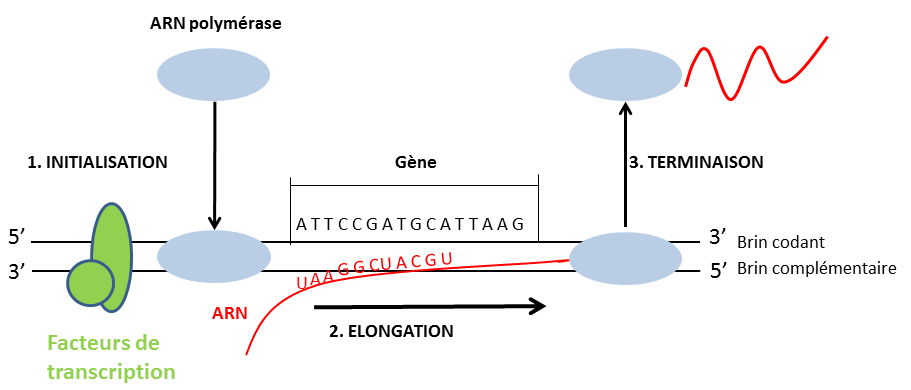
\includegraphics[scale=0.7]{Figures/transcription.png}
\caption{Le déroulement de la transcription chez les eucaryotes}
\label{trans}
\end{figure}

Durant l'initialisation, les facteurs de transcription se fixent aux TFBS et recrute l'ARN polymérase. Le brin d'ADN matrice est transcrit en ARN au moment de la phase d'élongation, le brin d'ARN sera constitué des bases complémentaires à celle de l'ADN (A $\rightarrow$ Uracile(U), \\C $\rightarrow$ G, T $\rightarrow$ A). La terminaison correspond au détachement de l'ARN polymérase, ce qui entraîne la libération du brin d'ARN nouvellement synthétisé.

La transcription est un processus régulé par différents éléments qui contrôlent son exécution. Les TFBS sont impliqués dans ces régulations en permettant la fixation des éléments régulateurs et nos analyses se focalisent sur ces éléments.

\subsubsection{Les facteurs de transcription : des éléments régulateurs} \label{subsec:regul}

Les séquences exprimées durant la transcription sont les gènes. Chacun contrôle un caractère particulier ce qui implique que leur expression varie en fonction du type cellulaire. Ce différentiel d'expression est, entre autres, permis par des éléments régulateurs de l'expression génique qui agissent à différents niveaux. Parmi les éléments régulateurs se trouvent les facteurs de transcription. Ces facteurs sont dépendant de sites de fixation se trouvant majoritairement en amont du gène : les TFBS.

\subsubsection{Les sites de fixation des facteurs de transcription}\label{subsec:TFBS}

Les facteurs de transcription régulent le recrutement du complexe d'initialisation de la transcription en se fixant sur des séquences d'ADN régulatrices : les TFBS. Ils peuvent être à proximité du promoteur ou bien plus éloigné (plusieurs milliers de paires de bases en amont du gène).

Les motifs de liaison aux TFBS des facteurs de transcription sont divers : doigt de zinc, hélice-boucle-hélice et leucine-zipper étant les trois principalement décrits. Ces motifs permettent aux facteurs de transcription de se fixer à l'ADN. Une boucle d'initialisation leur permettant ainsi d'agir avec le complexe d'initialisation est alors formée.

Les TFBS sont le point d'ancrage des facteurs de transcription. Chacun est associé à un ou plusieurs facteurs dont le rôle est d'activer ou d'inhiber des gènes. Un TFBS à donc une \gls{sequence nucleotidique} et une position spécifique qui permettent à ses facteurs de s'y fixer.

Des variations dans les TFBS peuvent entraîner une altération de la séquence et de la position et par conséquent une possible inactivation de ceux-ci. Inversement, certaines variations pourraient induire la formation de nouveaux TFBS. Lorsqu'un  TFBS est nouvellement activé, les facteurs qui lui sont associés vont s'y fixer et les gènes sur lesquels ils jouent un rôle pourraient alors être sur-exprimés ou, au contraire, sous-exprimés (de même pour la destruction d'un site). Dans le cas de modifications de la structure des TFBS, de nouvelles molécules pourraient se fixer et jouer un rôle différent, voir contraire, de celui du facteur se fixant originellement au TFBS.

Les variations peuvent être de plusieurs types : \og \acrlong{snp}\fg ~(\acrshort{snp}), insertion ou délétion de petites séquences nucléotidiques (\acrshort{indel}) comme le montre la figure \ref{snp}. Un SNP signifie qu'une base dans le génome étudié est différente de celle du génome de référence (hg19 ou GRCh37). On appel \gls{genome de reference}, un génome représentatif d'une espèce assemblé à partir de plusieurs génomes différents de cette même espèce. Un INDEL signifie que plusieurs bases ont été ajoutées (INsertion) ou supprimées (DELétion). Dans les cas de cancer, il peut être possible de comparer l'\gls{ADN constitutionnel} avec l'\gls{ADN tumoral}. Des mutations peuvent être trouvées à la fois dans l'ADN constitutionnel et tumoral, on parle de mutations constitutionnelles. D'autres peuvent être observées uniquement dans l'ADN tumoral, on parle de  mutations somatiques comme l'illustre la figure de l'annexe \ref{fig:somatique}.

\begin{figure}[h]
\centering
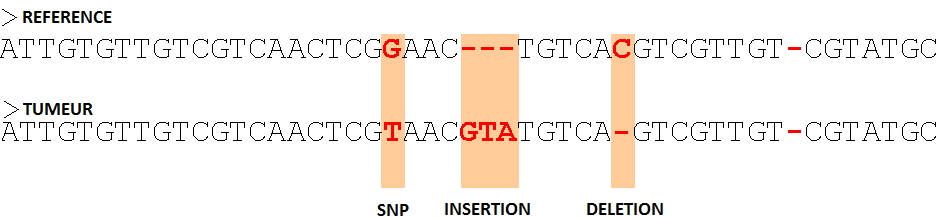
\includegraphics[scale=0.6]{Figures/indel_snp.png}
\caption{Illustration d'un SNP, d'une délétion et d'une insertion}
\captionsetup{font={footnotesize,bf,it}}
\caption*{D'après : http://sniplay.southgreen.fr/cgi-bin/documentation.cgi}
\label{snp}
\end{figure}

Des modifications similaires à celle de la figure \ref{snp} pourraient déréguler les processus de la transcription (initialisation, élongation et terminaison). Les informations génétiques présentes dans l'ADN ne seraient alors pas transcrites convenablement.

\subsection{Les données ICGC}\label{subsec:NGS}

Les données utilisées dans le projet SFT de l'ICGC sont issues de prélèvements de cellules tumorales (échantillons d'ADN et d'ARN tumoraux) et de prélèvements sanguins (échantillons d'ADN constitutionnel). Actuellement, 80 échantillons tumoraux ont été prélevés sur 68 patients atteints de LMS au sein de l'institut Bergonié et de plusieurs autres centres partenaires à travers la France. Les séquences d'ADN contiennent toutes les informations génétiques d'un individu, elles ont donc été extraites par des techniques séquençage NGS. Ce séquençage a été réalisé à une profondeur de 30X pour les échantillons constitutionnels et 50X pour les échantillons tumoraux. 

Les différents échantillons proviennent des trois principales localisations : intra-abdominal (58\%), membre (30\%), utérin (12\%). Afin d'accéder à l'hétérogénéité tumorale, deux échantillons ont été séquencés à une profondeur plus élevée : 200X pour la tumeur et 50X pour le constitutionnel, et six autres ont été séquencés à des localisations différentes (de 2 à 6 fragments) dans la tumeur. Le séquençage de plusieurs échantillons provenant de la même tumeur mais de localisations différentes permettra l'étude de l'évolution tumorale.

On définit la profondeur comme étant la couverture minimale de chacune des bases de la molécule d'ADN. Ainsi, une profondeur de 5X signifie que chaque base est couverte par au minimum 5 bases provenant de 5 séquences différentes comme l'illustre la figure \ref{depth}.

\begin{figure}[h]
\centering
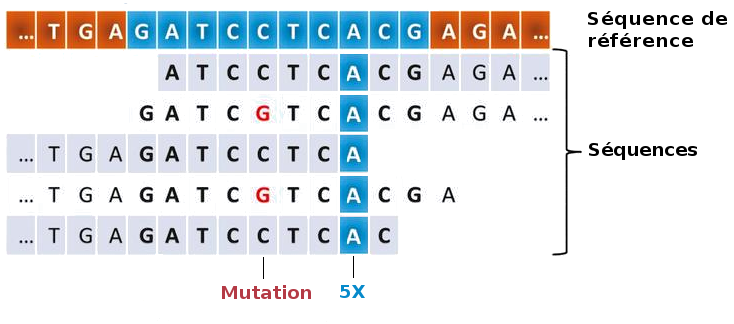
\includegraphics[scale=0.6]{Figures/depth.png}
\caption{Profondeur de séquençage après alignement}
\captionsetup{font={footnotesize,bf,it}}
\caption*{D'après : Diagnostic use of Massively Parallel Sequencing in Neuromuscular Diseases: Towards an Integrated Diagnosis}
\label{depth}
\end{figure}

Les séquences obtenues se présentent sous la forme de fichiers plats au format FastQ. Ces fichiers ne sont pas exploitables directement pour la détection de variants. Ils sont donc alignés avec le logiciel \textbf{Bowtie2} \citep{Bowtie}. Ce logiciel a été retenu en raison de sa rapidité et de sa haute performance dans le domaine de l'alignement global. L'alignement est réalisé  à partir d'un fichier FastQ et d'un fichier Fasta correspondant au génome de référence. Des fichiers au format \og \acrlong{sam}\fg  ~(\acrshort{sam}) dont la taille est très importante (plus de 100 Gigabit (Gb)) sont générés, ils sont alors compressés, en format binaire : le \og \acrlong{bam}\fg ~(\acrshort{bam}).

Une étape de post-alignement a été réalisée pour éliminer les \gls{sequences dupliquees} c'est-à-dire les séquence ayant les mêmes positions de départ et de terminaison.

L'analyse des données RNA-Seq a été réalisée avec la suite de logiciels TopHat2 \citep{Tophat} et Cufflinks \citep{Cufflinks}. Ce logiciel permet d'assembler les transcrits, de calculer leur abondance et de tester les différentiels d'expression. Un fichier contenant les valeurs normalisée en \og Fragment Per Kilobase Of Exon Per Millon Fragments Mapped\fg ~(FPKM) de l'expression des gènes a été généré pour chaque échantillon.

\newpage
\section{La détection de variants}\label{sec:detection}

La caractérisation des mutations somatiques des TFBS dans le génome des LMS implique de faire des choix parmi tous les outils existants. En effet, ils ne détectent pas tous les mêmes types de variants : SNP, INDEL... et présentent des caractéristiques différentes

\subsection{Les logiciels de modification de fichiers}\label{subsec:manip}

Afin d'utiliser les logiciels de détection, des modifications de fichiers comme des conversions de format par exemple, peuvent être nécessaires. Ces modifications étant courantes dans les analyses de type NGS, plusieurs logiciels ont été développés.

\subsubsection{Picardtools}

Ce logiciel est composé de nombreux outils aux utilisations diverses. Ces outils permettent de manipuler et d'extraire des informations des fichiers de données  (aux formats SAM ou BAM) provenant d'alignement de séquences \citep{Picard}.
\paragraph*{\textit{AddOrReplaceReadGroups}} ~permet d'ajouter les \og \gls{read group}\fg , il peut être utilisé avec les options VALIDATION\_STRINGENCY qui valide chaque séquence, SORT\_ORDER qui trie dans l'ordre des coordonnées et CREATE\_INDEX qui crée des index (description du fichier).
\paragraph*{\textit{ReorderSam}} ~permet de réorganiser le fichier suivant l'\gls{ordre caryotypique}  c'est-à-dire du chromosome 1 au 22 puis X, Y et Z.  Les mêmes options que celles d'\textit{\textbf{AddOrReplaceReadGroups}} sont disponibles.
\paragraph*{\textit{MarkDuplicate}} ~quant à lui sert à éliminer toutes les séquences dupliquées.

\subsubsection{VCFtools} 
Ce logiciel permet de manipuler les fichiers au format  \acrlong{vcf} ~(\acrshort{vcf}) \citep{VCF}. Les fichiers donnés en entrée doivent être compressés avec \textbf{bgzip} et l'indexation doit être réalisée avec \textbf{tabix}.

\paragraph*{\textit{vcf-sort}} ~permet de trier les données.
\paragraph*{\textit{vcf-concat}} ~permet de concaténer plusieurs fichiers, l'option -f sert à donner un fichier contenant le nom de tout ceux que l'on souhaite concaténer.
\paragraph*{\textit{vcf-merge}} ~permet de faire la fusion de plusieurs fichiers, l'option -d permet de supprimer les lignes dupliquées.
\paragraph*{\textit{vcf-isec}} ~permet de faire une intersection de deux fichiers ou plus avec l'option -n.

\subsubsection{BCFtools}

Ce logiciel permet de manipuler des fichiers VCF compressés en format BCF \citep{BCF}. L'utilisation de fichiers compressés augmente la rapidité des outils. 

\paragraph*{\textit{sort}} ~permet de trier les données.
\paragraph*{\textit{merge}} ~permet de fusionner plusieurs fichiers, l'option -d permet de supprimer les lignes dupliquées.
\paragraph*{\textit{isec}} ~permet de faire une intersection de deux fichiers ou plus avec l'option -n.
\paragraph*{\textit{query}} ~permet d'extraire des champs dans un autre fichier, l'option -f sert à préciser le format.

\subsubsection{Bedtools}

Ce logiciel permet de manipuler les fichiers au format \og \acrlong{bed}\fg ~(\acrshort{bed}), \og \acrlong{gff} \fg ~(\acrshort{gff}), BAM et VCF \citep{bedtools}. 
\paragraph*{\textit{intersect}} ~permet de faire l'intersection de plusieurs fichiers. L'option -header de cet outil sert à générer un fichier VCF à partir de deux fichiers de ce même type.

\subsubsection{Samtools} 

Ce logiciel permet de manipuler des fichiers d'alignement au format SAM/BAM ou \acrshort{cram} \citep{Samtools}.
\paragraph*{\textit{view}} ~sert à extraire des données comme par exemple l'extraction des données associées aux TFBS, les options -b et -o permettent de sortir le nouveau fichier au format BAM, les options -H et -h permettent d'isoler les \og header\fg ~et l'option -R de donner une région (ou un fichier de région).
\paragraph*{\textit{index}} ~sert à indexer les fichiers.
\paragraph*{\textit{mpileup}} ~quant à lui permet de générer des fichiers plats contenant la description de chaque base du génome. La qualité d'alignement minimum des séquences peut être filtrée avec l'option -q, l'option -B sert à supprimer le \og base alignment quality\fg (BAQ) qui calcule la probabilité qu'une séquence soit mal alignée et l'option -f sert à préciser le chemin d'accès au fichier de référence.

\subsubsection{Genome Analysis Toolkit (GATK)} 

Ce logiciel permet de manipuler plusieurs types de fichiers (BAM, VCF, etc.). \paragraph*{\textit{RealigneTargetCreator}} ~et \textbf{\textit{IndelRealigner}} servent à ré-aligner les bases autour des INDEL afin de supprimer au maximum les erreurs liées au séquençage. 
\paragraph*{\textit{BaseRecalibrator}} ~et \textbf{\textit{PrintReads}} s'associent pour éliminer les erreurs liées à l'alignement. Le premier permet de calculer un score de qualité (nombre de \og mismatch \fg ~par rapport à la référence). Un \og mismatch \fg ~signifie que la base trouvée dans le génome de référence est différente ou inexistante dans le génome tumoral. Toutes les séquences dont le score de qualité est inférieur à Q20 (plus d'1\% de \og mismatch \fg) sont éliminées. Le second sert à ajouter le score calculé précédemment et à générer un fichier BAM qualifié de recalibré. Tous ces outils sont parallélisables par des options ou par l'outil \textbf{Queue} développé par le \textit{Broad Institute}.\\
\paragraph*{\textit{\textbf{AnalyzeCovariates}}} ~sert à comparer les résultats avant et après le recalibrage des bases.

\newpage
\subsection{Les logiciels de détection de variants}\label{subsec:caller}

Dans le domaine de la génétique, la détection de variants est une étape incontournable des analyses. De nombreux logiciels ont donc été développés dans ce sens.

\subsubsection{Samtools}\label{sam}

Ce logiciel est composé de nombreux outils comme vu dans la partie \ref{subsec:manip}. \textbf{\textit{view}} et \textbf{\textit{mpileup}} peuvent être utilisés pour faire de la détection de variants en les associant avec d'autres outils comme ceux de \textbf{BCFtools}. 

Tous les outils de samtools disposent d'une palette d'options qui n'ont aucune valeur par défaut. Ainsi chaque utilisateur doit définir ses propres paramètres et adapter son analyse à ses données.

\subsubsection{Genome Analysis Toolkit}\label{GATK}

\textbf{GATK} est un logiciel développé par le \og Data Science and Data Engineering group\fg ~au sein du \textit{Broad Institute} ~\citep{GATK1}. Ce logiciel est composé de nombreux outils aux applications diverses.

Parmi les nombreux outils fournis dans GATK se trouvent des outils de détection de variants somatiques. 

\paragraph*{HaplotypeCaller} ~est un outil permettant de détecter les variations de type SNP et INDEL dans la \gls {lignee germinale}. Il réalise un réalignement local des haplotypes (groupes d'allèles situés sur un même chromosome à des positions différentes) dans les régions actives. Le logiciel commence par détecter les régions actives (régions pour lesquelles il y a des variations). Il construit ensuite un graphe de De Bruijn pour ré-assembler les régions actives et identifie les possibilités qu'il y ait des haplotypes dans les données.

\paragraph*{MuTect} ~permet de détecter les variations somatiques à partir de données issues de techniques de séquençage NGS et alignées \citep{Mutect}. Il prend en entrées trois fichiers d'alignement de séquence au format BAM : un tumoral et un constitutionnel, ainsi qu'un fichier de référence pour réaliser la détection de variants. 

\paragraph*{MuTect} ~se déroule en trois étapes :
\begin{itemize}
\item Preprocessing : alignement des séquences provenant des deux fichiers d'entrée.
\item Analyse statistique : identifier les sites portant des variations somatiques (utilisation des deux équations Bayesiennes). L'équation \ref{tumor} permet de vérifier qu'un site trouvé dans la tumeur n'est pas dans la référence, et la \ref{normal} vérifie que l'allèle variant n'est pas dans l'échantillon constitutionnel.

\begin{equation}\label{tumor}
\small LOD_{T} = log_{10} \frac{P(nombre ~de ~sites ~dans ~la ~tumeur|nombre ~de ~sites ~\textit{mutés})}{P(nombre ~de ~sites ~dans ~la ~tumeur | nombre ~de ~sites ~dans ~la ~\textit{référence})}
\end{equation}

\begin{equation}\label{normal}
\small LOD_{C} = log_{10} \frac{P(nombre ~de ~sites ~dans ~le ~constit|nombre ~de ~sites ~dans ~la ~\textit{référence})}{P(nombre ~de ~sites ~dans ~le ~constit | nombre ~de ~sites ~\textit{mutés})}
\end{equation}

\item Post-processing : nettoyage des données (suppression des artefacts liés au séquençage, des petites séquences ...) et génération d'un fichier au format VCF.
\end{itemize}

\subsubsection{Varscan}\label{subsec:varscan}

Ce logiciel de détection de variants permet d'identifier les variations somatiques et le nombre de copie (\og \gls{copy number}\fg) ~au sein d'un jeu de données \citep{Varscan}. Les fichiers d'entrée utilisés par le logiciel \textbf{Varscan} doivent être au format mpileup.

Les paramètres par défaut de \textbf{Varscan} permettant de déterminer si un variant est somatique ou non sont de 8 séquences couvertes pour l'échantillon constitutionnel et de 6 pour l'échantillon tumoral. Il est possible de jouer sur ces paramètres lors du lancement initial afin de filtrer les éléments détectés. Il génère deux fichiers de sortie contenant toutes les variations détectées, un pour les SNP et un autre pour les INDEL. 

\paragraph*{\textit{ProcessSomatic}} ~est un outil qui permet de séparer les variations selon leur type : perte de l'hétérozygocité (\acrshort{loh}), lignée germinale (Germline) ou Somatique (Somatic). Il est ainsi possible de ne conserver que les variations somatiques. Cet outil permet également de séparer les variations en fonction de leur fréquence allélique c'est-à-dire de leur fréquence d'apparition. Il ne conserve que les variations dont la fréquence allélique est inférieure à 5\% pour l'échantillon constitutionnel et minimum égale à 10\% pour l'échantillon tumoral. 

\subsubsection{Atlas2}\label{Atlas}

Ce logiciel de détection de variants permet d'identifier les variations de type SNP et INDEL dans des fichiers d'alignements d'exomes \citep{Atlas}. Il est capable de reconnaître les vrais positifs et les erreurs liées au séquençage ou à l'alignement des séquences en utilisant un modèle de régression logistique ayant suivi un processus de \og \gls{machine learning}\fg. Deux modules sont utilisés pour la détection.

\paragraph{\textit{Atlas-SNP2}} ~sert à détecter les variations de type SNP.
\paragraph{\textit{Atlas-Indel}} ~sert à détecter les variation de type INDEL. 

Les données séquencées par les plates-formes suivantes peuvent être utilisées en paramètre d'entré pour Atlas2 : SOLID, Illumina et Roche 454.

Des fichiers tabulés, au format VCF, sont produits. Ils contiennent les SNP et les INDEL détectés.

\paragraph{\textit{vcfPrinter}} ~sert à rassembler plusieurs fichiers VCF en un seul. L'option -indel permet de spécifier que les fichiers contiennent des INDEL. Une option dont le but est d'augmenter la rapidité peut être placée en paramètre avec l'option -fast, elle est plus efficace avec une vingtaine de fichiers au maximum et des sites de 50000 paires de bases.

\subsubsection{SomaticSniper}\label{Somatic}

Ce logiciel détecte les variants de type SNP \citep{Sniper}. Il prend en entrée deux fichiers au format BAM, l'un contenant la séquence tumorale et l'autre la séquence constitutionnelle, et un fichier de référence au format FASTA. Il compare les deux fichiers avec la référence et ressort les positions auxquelles un SNP est observé dans un autre fichier tabulé. L'option -F permet de spécifier le type VCF comme format de sortie, l'option -Q permet de filtrer les SNP en donnant une valeur de qualité (15 par défaut) à partir de laquelle le SNP est considéré comme somatique.

Ce logiciel permet de calculer la probabilité que les génotypes tumoraux et constitutionnels soient différents. Il retourne cette probabilité sous forme d'un score entre 0 et 255, 0 signifiant que les génotypes sont identiques et 255 qu'ils diffèrent énormément.

\subsubsection{Récapitulatif}

Les logiciels de détection de variants sont nombreux, certains ayant été développés pour le traitement de données NGS (MuTect, Varscan, SomaticSniper) tandis que d'autres ont été au départ développés pour d'autres utilisations comme la modification de fichiers (Samtools). 

\begin{table}[h]
\centering
\begin{tabular}{|c|c|c|c|c|c|c|}
\hline
Logiciel & Mise à jour & SNP & INDEL & Somatique & Parallélisable \\
\hline
Samtools & 04/2016 & \textbf{OUI} & \textbf{OUI} & non  & non\\
\hline
MuTect & 02/2016 & \textbf{OUI} & \textbf{OUI} & \textbf{OUI} & \textbf{OUI}\\
\hline
Atlas2 & 03/2013 & \textbf{OUI} & \textbf{OUI} & non & non\\
\hline
SomaticSniper & 07/2015 & \textbf{OUI} & non & \textbf{OUI} & non\\
\hline
Varscan2 & 06/2015 & \textbf{OUI} & \textbf{OUI} & \textbf{OUI} & non\\
\hline
\end{tabular}
\caption{Récapitulatif des caractéristiques de chaque logiciel}
\label{caract}
\end{table}

La tableau \ref{caract} présente les différentes caractéristiques de chaque logiciel décrit dans la partie \ref{subsec:caller}. Il est intéressant de noter qu'un des outils est parallélisable ce qui permet d'augmenter sa vitesse d'exécution, point non négligeable lors de l'analyse de grandes masses de données.

Les outils choisis vont permettre de détecter un maximum de variants. Cependant, les logiciels de détections ne permettent pas de caractériser ces derniers. Une annotation doit donc suivre l'étape de détection.

\section{L'annotation des variants}\label{annotation}

L'annotation a pour but de documenter le plus précisément possible un génome, un transcriptome ou une variation de séquence. Au vu du nombre de données qui s'accroît, des algorithmes d'annotation automatique ont vu le jour. Ces algorithmes se basent sur la correspondance entre les données issues d'une base et celles provenant du fichier à annoter.

Les bases de données, diverses et variées permettent de choisir le type d'éléments que l'on souhaite annoter. Dans le cadre de ce projet, les variations des TFBS doivent être annotées, il faut donc trouver une base de données regroupant les TFBS ou plus généralement les régions régulatrices.

Dans leur étude sur les mutations somatiques récurrentes des régions régulatrices \citet{Melton} ont utilisés les bases de données \textbf{RegulomeDB} pour annoter les régions régulatrices du génome et \textbf{Genecode17} pour annoter des transcripts. Cependant, il existe de nombreuses autres bases.

\subsubsection{Les bases de données}\label{subsec:bdd}
\paragraph{1000 genomes} ~ou \textbf{1000G} est une base de données constituée à partir du séquençage du génome complet de plus de 1000 individus \citep{1000} provenant du monde entier. Elle est téléchargeable sur le site du projet 1000 genomes \citep{genome} et la dernière version date de mai 2015. Une extension de cette base est en cours avec le séquençage des génomes de 100 000 individus \citep{100000}. 

\paragraph{Mills}, ~d'après le nom de son auteur, est une base de données construite dans le cadre du même projet que 1000G et téléchargeable à la même adresse. Elle se compose d'un jeu de données d'INDEL validés séparément de celui de 1000G. La dernière mise à jour de la base date de 2013 \citep{mills}.

\paragraph{dbSNP} ~est une base de données constituée de toutes les variations génétiques qui ont pu être détectées lors de travaux de recherches \citep{dbsnp}. Tous les utilisateurs peuvent écrire dans cette base, les données présentes n'ont donc pas nécessairement été validées biologiquement avant d'être incluses dans la base. La version 147 est parue en avril 2016.

\paragraph{RegulomeDB} ~proposée par \textbf{ENCODE} se présente sous la forme d'une application web utilisant une base de données avec des informations sur les régions régulatrices \citep{Regulome}. La base utilisée pour l'annotation provient de dbSNP141 elle date donc de mai 2014.

\paragraph{Genecode} ~est une base de données, contenant toutes les informations sur les gènes, obtenues en combinant une annotation manuelle \textbf{HAVANA} ~\citep{Havana} et une annotation automatique faite par \textbf{Ensembl} \citep{Gencode}. La dix-neuvième version est parue en août 2015, elle a été mise à jour avec la nouvelle annotation d'\textbf{HAVANA}, la version 74 du jeu de gènes d'\textbf{Ensembl} du génome humain (hg19).

\paragraph{tfbsConsSites} ~est une base de données des TFBS mise à jour avec les données de \textbf{TRANSFAC} et proposée par \textit{l'UCSC}\cite{UCSC}. Les données de \textbf{TRANSFAC} sont mise à jour une fois par an (dans la version commercial du projet) et vérifiées biologiquement \citep{Transfac}. La dernière version libre d'accès disponible de cette base date de 2011 alors que \textbf{TRANSFAC} a été mise à jour en janvier 2016 dans sa version commerciale.

\paragraph{JASPAR} ~est une base de données des TFBS  constituée de profils permettant une représentation graphique des TFBS réalisée à partir de \og \acrlong{pwm}\fg ~(\acrshort{pwm}) \citep{Jaspar}. Ces PWM sont obtenues à partir d'une matrice composée du nombre d'occurrences de chaque nucléotide dans la séquence. La dernière mise à jour disponible de \textbf{JASPAR} date de 2014.

\paragraph{OregAnno} ~est constituée de régions régulatrices, de TFBS, de sites de fixation de l'ARN et d'autres éléments régulateurs identifiés de façon expérimentale \citep{Oreg}. Elle a été mise à jour pour la dernière fois en décembre 2015.

\paragraph{wgEncoderegtfbs} ~est une base de données proposée par ENCODE et disponible sur le site de l'UCSC. Cette base est constituée des TFBS identifiés durant le projet ENCODE à partir d'un grand jeu de données Chip-Seq \citep{wgEncode}. La dernière date de mise à jour est d'août 2013.

\subsubsection{Les outils d'annotation}

Le choix des outils d'annotation et du jeu de données peut avoir un impact sur le résultat de l'annotation comme le démontre l'article de \citet{annot}. Deux outils d'annotation populaires ont été comparés \textbf{Annovar} et  \textbf{Variant Effect Predictor} (VEP) dans le cadre de cet article.

\paragraph{Annovar} ~est un logiciel permettant d'annoter les mutations SNP et INDEL détectées en fonction de gènes, de régions ou en utilisant des filtres (dbsnp, etc.) \citep{Annovar}. Ce logiciel propose l'utilisation d'une palette de bases de données parmi lesquelles on retrouve \textbf{tfbsConsSites} pour l'annotation des TFBS. Il est cependant possible d'utiliser n'importe quelle base de données au format tabulé composée des trois  colonnes : Chromosome, Position initiale et  Position terminale. Ce logiciel prend un fichier tabulé en entrée et engendre un fichier du même type en sortie qui contiendra toutes les entrées qui chevauchent les entrées de la base de données utilisée. Plusieurs scripts écrit en perl sont disponibles dans \textbf{Annovar} pour convertir les données d'un format à un autre, faire de l'annotation simple (avec une seule base de données) ou multiple (plusieurs bases de données en même temps),etc. Ce logiciel est mis à jour plusieurs fois par an et la dernière mise à jour date de février 2016.

\paragraph{VEP} ~est un logiciel d'annotation proposé par \textbf{Ensembl} \citep{ensembl} qui permet d'annoter les variants et de déterminer les effets qu'ils ont sur les transcripts et les protéines des jeux de données Gencode, Ensembl transcripts et RefSeq transcripts \citep{Refseq}. Il prend en entré un fichier tabulé et en génère un nouveau en sortie dans lequel on trouve des entrées d'éléments régulateurs, de transcripts, etc. Il est possible d'extraire du fichier de résultats uniquement les lignes concernant les variants des régions régulatrices. VEP met également à disposition un outil de représentation graphiques des résultats obtenus. Cet outil a été mis à jour en septembre 2015.

\paragraph{R} ~est un logiciel de statistique \citep{R} ~qui permet également de faire de l'annotation de variants en associant le package \og VariantAnnotation \fg ~de Bioconductor et des bases de données. Ce package permet de passer en entrée des fichiers VCF \citep{Rpack}. L'annotation est alors faite sur ces fichiers avec la  ou les base(s) choisie(s). Ce package a été mis à jour pour la dernière fois en mai 2016.

\paragraph{VariantAnnotator} ~est un outil d'annotation proposé par le logiciel GATK \citep{GATK}. Il permet d'annoter les variants selon leur contexte et non de façon fonctionnelle (plus classique). L'option -dbsnp permet d'annoter suivant les valeurs de la base dbSNP, -A sert à utiliser la profondeur de couverture. L'option -E permet de donner une expression particulière sur laquelle annoter (ex : la \gls{frequence allelique}). Il prend en entré un fichier BAM, des fichiers VCF pour les options et génère un fichier VCF en sortie. La dernière mise à jour date de novembre 2015.

\paragraph{Oncotator} ~est un logiciel développé par le \textit{Broad Institute} qui permet d'annoter des points de mutations et des INDEL de petites tailles \citep{oncotator}. L'annotation classe les variants suivant leur nom et produit des liens vers des données spécifiques du cancer provenant de ressources comme le TCGA \citep{TCGA} ou COSMIC \citep{cosmic}. La dernière version en date est sortie en avril 2016.
\chapter{Conception}

Les données brutes sur lesquelles le pipeline d'analyse est développé ont déjà subi une étape de pré-traitement durant laquelle les adaptateurs et les séquences d'une qualité inférieure à 20 ont été supprimés et les séquences chevauchantes ont été scindées en deux parties. Ces données ainsi nettoyées ont été alignées et servent d’entrées pour le pipeline d'analyse. Le développement du pipeline d'analyse se focalise donc sur la détection de variants. 

Lors de ce stage, les variations des TFBS doivent être isolées du reste des données. L'extraction de ces variations implique le développement d'un pipeline d'analyse. Il commence par une réorganisation des données afin de limiter les erreurs liées au séquençage et à l'alignement des séquences.

Les pipelines d'analyses spécifiques aux données NGS se construisent suivant un ordre précis décrit dans la publication de \citet{ref7}.

Quatre grandes étapes sont indispensables lors de l'analyse des données :
\begin{itemize}[label=\textbullet]
\item Organiser les données
\item Détecter les variants
\item Annoter les variants
\item Filtrer les résultats 
\end{itemize}

La figure \ref{fig:pipeline} ci-dessous, illustre le pipeline d'analyse élaboré, dans le but d'extraire toutes les variations des TFBS des différents échantillons de LMS disponibles. 

\begin{figure}[h]
\centering
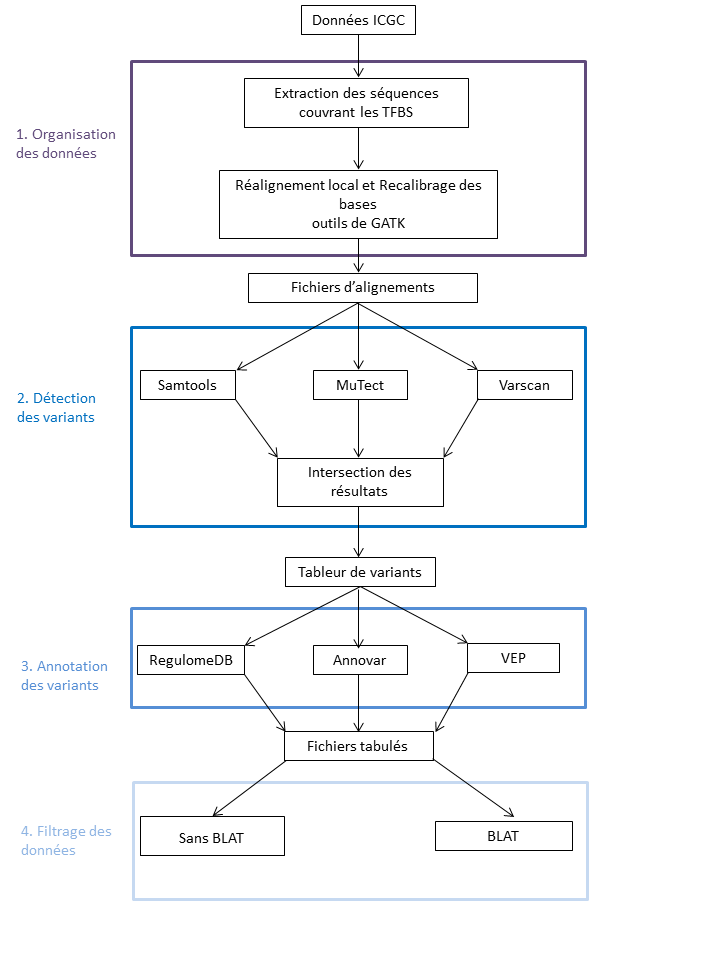
\includegraphics[width=10cm,height=11cm]{Figures/pipeline.png}
\caption{Pipeline d'analyse des données de l'ICGC}
\label{fig:pipeline}
\end{figure}

\section{Organisation des données}\label{sec: orga}

Les données issues de techniques de séquençage NGS de génomes complets sont très volumineuses, il est donc intéressant de les scinder en fonction des besoins. La figure \ref{fig:part1} montre la première partie du pipeline d'analyse. Dans cette partie les données seront extraites puis nettoyées.

\begin{figure}[h]
\centering
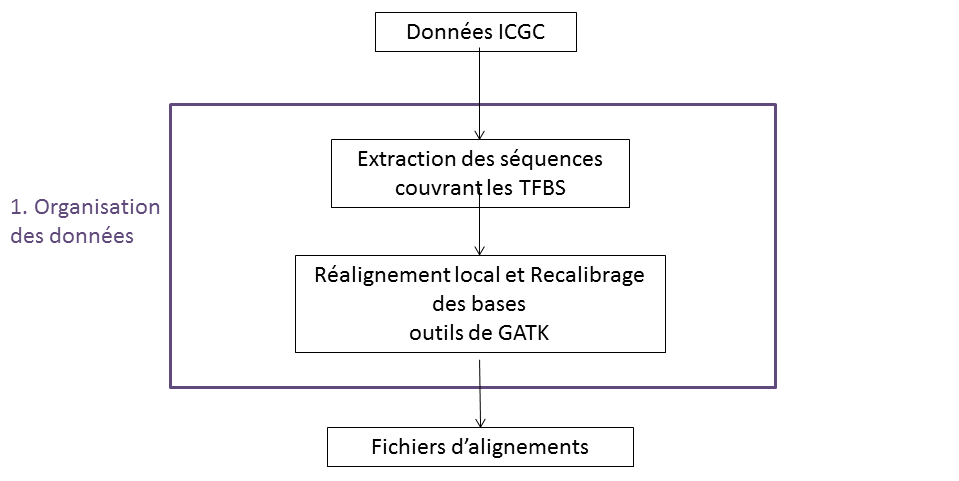
\includegraphics[scale=0.6]{Figures/partie1.png}
\caption{Réorganisation des données}
\label{fig:part1}
\end{figure}

Dans le cadre de ce projet de stage, je focaliserai mes analyses uniquement sur l'étude des TFBS. L'outil \textit{\textbf{view}} du logiciel \textbf{Samtools} pourra être utilisé pour extraire les séquences qui les recouvrent du reste du fichier d'alignement. Les options -H et -R sont passées en paramètres.

Les \og read group\fg ~n'ont pas été ajoutés lors de l'alignement des séquences (pas d'utilité pour l'équipe au moment de leur génération) or ils sont nécessaires au fonctionnement de logiciels d'alignement (MuTect, Varscan). L'outil \textit{\textbf{AddOrReplaceReadGroups}} de \textbf{Picartools} semble être utilisable pour les ajouter. Dans le but d'accélérer le processus, les paramètres suivant pourraient être donnés en entrées VALIDATION\_STRINGENCY = SILENT pour éviter les tests de validation des séquences, SORT\_ORDER = coordinate pour trier le fichier de sortie suivant ses coordonnées et CREATE\_INDEX = True pour créer un index du fichier de sortie.

Un second outil du même logiciel, \textit{\textbf{ReorderSam}}, pourra être mis à contribution pour réordonner les fichiers dans l'ordre caryotypique. Ce nouveau fichier ne sera pas indexé car l'utilisation de l'option qui le permet augmente le temps d'exécution. Pour l'indexer, l'outil \textit{\textbf{index}} du logiciel \textbf{Samtools} sera privilégié en raison de sa rapidité d'exécution.

Les fichiers réorganisés doivent passer par une étape de traitement supplémentaire pour éliminer le maximum d'erreurs liées au séquençage ou à l'alignement. Parmi tous les logiciels de manipulation des données présentés dans la partie \ref{subsec:manip}, un seul a été retenu : \textbf{GATK}. Les outils \textit{\textbf{RealigneTargetCreator}}, \textit{\textbf{IndelRealigner}}, \textit{\textbf{BaseRecalibrator}} et \textit{\textbf{PrintReads}} de ce logiciel pourront être mis à contribution lors de cette étape.

\newpage
\subsection{Le traitement par GATK}\label{sec: GATK}

Lors du séquençage, des erreurs liées à la technique utilisée ont pu être imprimées dans les fichiers de sortie. Il est donc important d'éliminer au maximum ces erreurs potentielles. Les concepteurs de GATK conseillent de passer les bases de données \textbf{Mills} et \textbf{1000G} aux outils \textit{\textbf{RealigneTargetCreator}} et \textit{\textbf{IndelRealigner}}. La base de données Mills est beaucoup plus restrictives que 1000G, elle ne sera donc pas conservées. La base de données 1000G peut être considérées comme robuste en raison du nombre important de données qui ont servis à la constituer bien que chaque donnée ne soit pas expérimentalement vérifiée. Elle sera donc conservée pour ces étapes.

Les erreurs liées au séquençage ne sont pas les seules, des erreurs liées à l'alignement des séquences peuvent exister. Les outils \textit{\textbf{BaseRecalibrator}} et \textit{\textbf{PrintReads}} de \textbf{GATK} pourront être mis à contribution pour les supprimer. Il est conseillé de passer, en supplément des deux bases Mills et 1000G, la base de données dbSNP dans une version supérieure à la 132. Pour les raisons citées dans le paragraphe précédent Mills n'est pas conservée. La base de donnée dbSNP contient un nombre très important de données cependant, toutes ces données n'ont pas été vérifiées expérimentalement. Du fait de cette information, cette base ne sera pas conservée. Ces outils disposent d'options de parallélisation (nombre de cpu, nombre de cœurs), elles pourront être prises en compte afin d'accélérer les processus d'exécution.

Des fichiers BAM ne contenant théoriquement plus d'erreur sont générés à la suite de ces deux étapes. Ces fichiers passent à l'étape suivante du pipeline : la détection des variants somatiques.

\section{Détection des variants somatiques}\label{sec:detec}

La seconde partie du pipeline est présentée dans la figure \ref{fig:part2}. Cette partie permettra de détecter les variants des TFBS.

\begin{figure}[h]
\centering
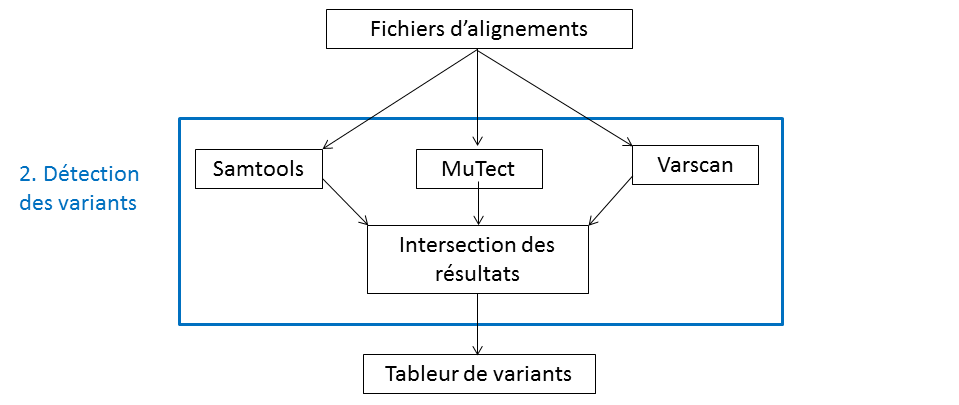
\includegraphics[scale=0.6]{Figures/partie2.png}
\caption{Détection des variants}
\label{fig:part2}
\end{figure}

Dans la partie \ref{subsec:caller} de l'analyse de ce sujet, plusieurs outils de détection de variants ont été examinés. Ces outils ne permettent pas tous de travailler simultanément sur plusieurs fichiers comme pour l'analyse comparative de données tumorales et constitutionnelles. 

\textbf{Atlas2} ne prend qu'un seul fichier en entrée, il ne peut donc pas comparer les séquences de l'échantillon tumorale avec celle de l'échantillon constitutionnel. Son utilisation nécessitant une étape de post-traitement, il ne sera pas conservé.

L'ensemble des données ayant déjà été généré avec \textbf{Samtools} par l'équipe, il sera conservé bien qu'il présente les mêmes caractéristiques qu'\textbf{Atlas2}.

\textbf{SomaticSniper} ne détecte que les SNP or pour analyser les variations des TFBS il faut également détecter les INDEL, il ne pourra donc pas être utilisé.

Une étude comparative de plusieurs outils de détection parmi lesquels se trouvent \textbf{Varscan} et \textbf{MuTect} \citep {Detecting} démontre que \textbf{Varscan} est le plus performant quand il s'agit de détecter des SNP de haute qualité (couverture et fréquence allélique prise en compte) et que \textbf{MuTect} au contraire détecte plus de SNP de basse qualité que les autres. Ces deux outils seront donc utilisés pour détecter les variants des TFBS. 

Les caractéristiques présentées dans le tableau \ref{caract} de l'analyse du sujet et les deux études précédemment citées permettent de sélectionner \textbf{MuTect} et \textbf{Varscan} comme logiciel de détection de variants pour la suite du pipeline. \textbf{Samtools} étant historiquement utilisé au sein de l'équipe et un certain nombre de données ayant déjà été calculées dessus, il m'a été demandé de l'intégrer comme un outil de mon pipeline.

\subsection{MuTect}

Lors de l'analyse du sujet, \textbf{MuTect} a été présenté comme comportant plusieurs filtres par défaut. Toutes les variations détectées ayant réussi à passer ces filtres sont étiquetées avec la valeur \og PASS\fg ~dans le champ \og FILTER\fg ~du fichier de sortie. Ces variations sont considérées comme somatiques. 

Le fichier de sortie est au format VCF, pour garder ce format il faudrait récupérer le header. L'outil \textit{\textbf{view}} du logiciel \textbf{Samtools} semble être applicable avec l'option -h pour extraire uniquement le header et le placer dans un fichier vide.

Dans le but de ne conserver que les variations somatiques, la commande \og grep \fg ~du shell linux pourrait être employée pour récupérer toutes les lignes étiquetées \og PASS\fg. Ces lignes seront conservées à la suite du fichier contenant le header, un nouveau VCF sera ainsi formé.

\subsection{Varscan}

Dans l'analyse du sujet, il est décrit que \textbf{Varscan} prend en entrée un seul fichier au format mpileup. Cependant, ce logiciel ne fournit aucun outil de transformation des fichiers BAM en mpileup. L'outil \textit{\textbf{mpileup}} de \textbf{Samtools} pourra être mis à contribution pour générer le fichier attendu. Les options -B pour supprimer le calcul de probabilité qu'une séquence soit mal alignée et -f pour donner la séquence de référence pourront être passées en entrées. L'option -q avec la valeur 1 qui permet de ne conserver que les séquence de qualité minimum 1 pourra également être utilisée.

Dans la partie \ref{subsec:varscan} il a été vu que deux fichiers VCF sont générés par \textbf{Varscan}. L'outil \textit{\textbf{ProcessSomatic}} pourra être mis en application sur chacun de ces fichiers afin de séparer les variations somatiques des autres variations LOH et germinales.

L'extraction va de nouveau produire quatre fichiers, deux pour les SNP, un avec les variations de haute qualité et un second avec les autres, et deux pour les INDEL, un avec les variations de haute qualité et un avec les autres. L'outil \textit{\textbf{vcf-concat}} du logiciel \textbf{VCFtools} pourra être utilisé afin de les rassembler en un seul fichier qui contiendra les SNP et les INDEL de haute qualité. Ce fichier pourra alors être fusionné avec celui généré par \textbf{MuTect}

\subsection{Samtools}\label{subsec:sam}

Le logiciel Samtools permet de faire de la détection de variants cependant il doit être associé à un autre logiciel, \textbf{BCFtools}.

Un pipeline de détection de variants réalisé avec Samtools a déjà été développé par l'équipe de l'institut Bergonié. Ce pipeline permet de détecter toutes les variations présentes dans un jeu de données. Cependant les variations détectées ne sont pas toutes somatiques. Il faudra donc appliquer des filtres sur les données obtenues. 

Les filtres qui seront utilisés ont déjà été développés par \cite{Filtre}. Dans cet article, les auteurs partent du principe qu'une variation est somatique si la couverture minimale de l'échantillon constitutionnel est de 8 et celle de l'échantillon tumoral de 14 à cette position. Les variations dont la fréquence allélique est supérieure ou égale à 30\% sont conservées. 

\section{Annotation des variants}

Le processus d'annotation des variants permet de caractériser les différentes variations détectées d'après le processus de la partie \ref{sec:detec}. Plusieurs outils ont été présentés lors de l'analyse de ce sujet. La troisième partie du pipeline présentée sur la figure \ref{fig:part3} montre le cheminement du processus d'annotation.

\begin{figure}[h]
\centering
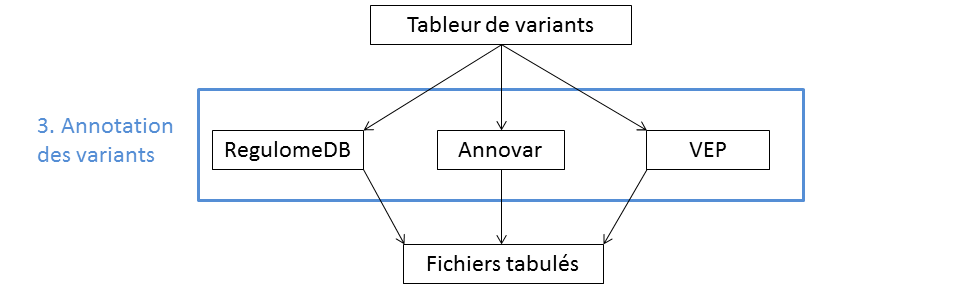
\includegraphics[scale=0.6]{Figures/partie3.png}
\caption{Annotation des variants}
\label{fig:part3}
\end{figure}

\subsection{Choix des logiciels}

Le logiciel \textbf{Annovar} permet d'utiliser de nombreuses bases de données lorsqu'elles sont formatées selon les exigences du logiciel. Il peut donc théoriquement utiliser n'importe quelle base de données. \textbf{Annovar} est très rapide, performant et régulièrement mis à jour. Il est donc retenu pour faire l'annotation des variants somatiques. Les scripts permettant de faire de l'annotation simple et multiple pourront être utilisés en fonction du nombre de base de données sélectionnées.

Le logiciel \textbf{VEP} est rapide et performant, il utilise des bases de données de transcrits comme \textbf{Gencode} pour annoter les variants. VEP peut détecter des variations dans les régions régulatrices, cependant il n'est pas possible de lui donner une base de données des TFBS, il ne détectera donc que ce qui se trouve dans les bases de données de transcrits qu'il utilise. Ce logiciel ne sera donc pas retenu pour réaliser l'annotation des variants somatiques des TFBS, il pourra cependant être utilisé pour annoter les transcrits.

Le logiciel \textbf{R} et son package \textit{\textbf{VariantAnnotation}} ne permettent d'utiliser qu'un nombre limité de base de données (SIFT et Polyphen), ils ne seront donc pas conservés pour annoter les variants.

L'outil \textit{\textbf{VariantAnnotator}} proposé par \textbf{GATK} annote les variants selon leur contexte. Il permet par exemple de ressortir la profondeur de couverture de chacun ou encore la fréquence allélique. Il ne permet en revanche pas d'annoter les variants avec une base de données, il ne sera donc pas conservé pour l'étape d'annotation des variants.

Le logiciel \textbf{Oncotator} développé par le \textit{Broad Institute} n'annote que les points de variations et les INDEL de petites tailles. Il présente l'avantage d'annoter les variants en fonction de leur nom et de produire des liens vers des données spécifiques du cancer. Cependant, cela implique que les variants détectés soient déjà connus or je ne peux en être sûre, c'est pourquoi je ne conserve pas ce logiciel.

\begin{table}[h]
\centering
\begin{tabular}{|c|c|c|c|c|}
\hline
Logiciel & Choix des bdd & TFBS & Fonctionnelle \\
\hline
Annovar & \textbf{OUI} & \textbf{OUI} & \textbf{OUI}\\
\hline
VEP & non & non & \textbf{OUI}\\
\hline
Oncotator & non & \textbf{OUI} & \textbf{OUI}\\
\hline
VariantAnnotator & \textbf{OUI} & \textbf{OUI} & non\\
\hline
VariantAnnotation & non & \textbf{OUI} & \textbf{OUI}\\
\hline
\end{tabular}
\caption{Récapitulatif du choix des logiciels d'annotation}
\end{table}

\subsection{Choix des bases de données}

L'application web \textbf{RegulomeDB} utilise une base de données \textbf{dbSNP} pour réaliser l'annotation des variants des régions régulatrices. Le format de RegulomeDB risque de rendre son utilisation très difficile si le nombre de variations est élevé, un script pourrait être réalisé afin d'utiliser l'application localement. Annotant toutes les régions régulatrices, cette base contient les TFBS et sera conservée.

La base de donnée des TFBS, \textbf{tfbsConsSites}, de l'\textit{UCSC} est formatée pour pouvoir être utilisée avec Annovar afin d'annoter les variations somatiques des TFBS. Toutes les données qui y sont intégrées doivent avoir été vérifiées expérimentalement auparavant, cette base est donc fiable bien qu'elle n'ait pas été mise à jour depuis 2011. Elle pourrait être utilisée conjointement avec \textbf{Annovar} pour annoter les données. 

\textbf{OregAnno} présente l'avantage de n'être constituée que de données identifiées de façon expérimentale. Cependant, elle regroupe à la fois les régions régulatrices, les TFBS, les sites de fixation de l'ARN et encore d'autres éléments régulateurs. Le nombre de TFBS que l'on y trouve n'est donc pas très élevé or ce sont eux sur lesquels se focalise mon analyse. Cette base ne sera donc pas conservée pour annoter les données.

\textbf{wgEncoderegtfbs} contient un nombre important de TFBS identifiés au cours du projet \textbf{ENCODE}, elle pourrait donc être retenue. Cependant elle n'a pas été mise à jour depuis 2013 et les données qu'elle contient n'ont pas été vérifiées expérimentalement. Elle ne sera donc finalement pas retenue.

\begin{table}[h]
\centering
\begin{tabular}{|c|c|c|c|c|c|}
\hline
Base de données & Vérifier & Formater & Propre TFBS\\
\hline
tfbsConsSites & \textbf{OUI} & \textbf{OUI} & \textbf{OUI}\\
\hline
dbSNP & non & \textbf{OUI} & non\\
\hline
OregAnno & \textbf{OUI} & \textbf{OUI} & non\\
\hline
wgEncoderegtfbs & non & \textbf{OUI} & \textbf{OUI}\\
\hline
\end{tabular}
\caption{Récapitulatif du choix des bases de données}
\end{table}

Les données obtenues après l'annotation des variants pourront être filtrées afin d'éliminer tous les \gls{faux positifs}. Un alignement entre la séquence de référence et la séquence mutée pourra être réalisé (BLAT) ou, des scripts seront écrits pour filtrer suivant la fréquence allélique par exemple. La figure \ref{fig:part4} présente les deux approches envisagées. 

\begin{figure}[h]
\centering

\includegraphics[scale = 0.6]{Figures/partie4.png}
\caption{Filtrage des données}
\label{fig:part4}
\end{figure}

\section{Caractérisation des variations}

Les données filtrées contiendront un nombre minimum de \og faux positifs\fg. Une étude plus approfondie des TFBS pourra alors être envisagée.

Dans un premier temps, il faudra récupérer les TFBS porteurs d'une variation, un shell script sera réalisé pour ce faire.

Les facteurs de transcriptions agissent généralement sur des gènes proches de leur TFBS. En utilisant la base de données \textit{\textbf{RefSeq}} et l'outil \textit{\textbf{intersect}} du logiciel \textbf{Bedtools}, il sera possible de récupérer le ou les gènes les plus proche de chacun des TFBS mutés. 

Les bases de données \textit{\textbf{TRANSFAC}} et \textit{\textbf{CHEA}} disponibles sur le site web \textbf{Harmonizome} \citep{harmonizome} contiennent les gènes cibles des facteurs de transcription. Ces bases pourront être utilisés pour extraire les gènes cibles du jeu de gènes obtenus avec \textbf{Bedtools}.

L'analyse des valeurs de d'expression normalisées en FPKM permettra par la suite de savoir si les gènes, qu'ils soient cible ou pas, ont un changement d'expression. 
 



\chapter{Réalisation}
%Tout doit être au présent

Dans l'optique de détecter toutes les variations somatiques des TFBS dans les LMS, j'utilise les logiciels \textbf{Mutect} et \textbf{Varscan}. L'utilisation de \textbf{Mutect} nécessite une organisation spécifique des données. J'utilise plusieurs outils pour formater les fichiers d'alignement suivant les exigences de celui-ci. Tous ces outils sont intégrés à un pipeline d'analyse développé en bash qui nécessite de nombreuses ressources en mémoire pour fonctionner de façon optimale.

L'équipe \textit{Génétique et biologie des sarcomes} de l'institut Bergonié travaille en collaboration avec le \textit{\acrlong{mcia}} (\acrshort{mcia}) \citep{MCIA} qui met à disposition de ses utilisateurs un serveur de calcul constitué de 264 noeuds de calculs ayant 48 Gb de mémoire chacun, 4 noeuds de calcul avec 512Gb de mémoire et 2 noeuds pour les outils de visualisation.

Les données issues de techniques de séquençage NGS de génomes complets étant très volumineuses (voir la partie \ref{subsec:NGS}), je dois optimiser le temps d'exécution de mon pipeline. J'utilise donc les ressources du \textit{MCIA} mises à ma disposition.

\section{Organisation des données}

Le but de mon projet est de rechercher les variations somatiques touchant les TFBS. La première étape de mon pipeline d'analyse est donc l'extraction des séquences chevauchant les TFBS dans les fichiers d'alignements.

J'utilise un des outil du logiciel \textbf{Samtools} et une base de données contenant les positions des TFBS pour extraire toutes les séquences chevauchantes. L'extraction réalisée, produit un fichier dont la taille est réduite de 90\%. Lors de l'extraction, \textbf{Samtools} récupère toutes les séquences qui chevauchent la séquence d'intérêt d'au moins une paire de base. Les séquences contenues dans le fichier d'alignement mesurent au maximum 101bp, lorsqu'une base est commune entre la séquence et la région du TFBS, la séquence est récupérée par le logiciel. Ainsi les séquences récupérées peuvent couvrir jusqu'à 100 pb de plus à gauche et 100 pb de plus à droite que la région d'intérêt comme l'illustre la figure \ref{fig:sequence}.

\begin{figure}[h]
\centering
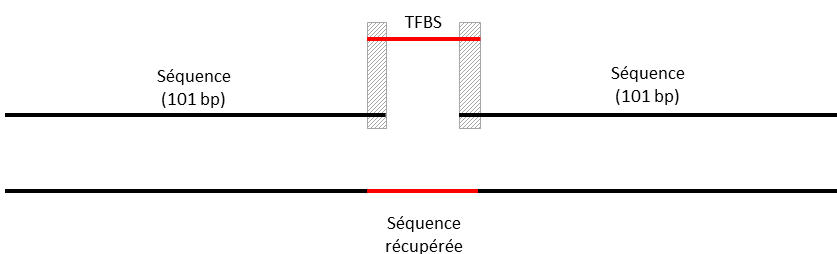
\includegraphics[scale=0.5]{Figures/sequence.png}
\caption{Fonctionnement de \textbf{Samtools}}
\label{fig:sequence}
\end{figure}

Pour utiliser les outils de \textbf{GATK} nécessaires à la détection de variants somatiques, un trie caryotypique des séquences contenues dans les fichiers d'alignement et un ajout des \og read group\fg ~est indispensable. J'utilise les outils \textit{\textbf{AddOrReplaceReadGroup}} et \textit{\textbf{ReorderSam}} du logiciel \textbf{Picardtools} pour trier et respectivement ajouter la nomenclature, selon les exigences de \textbf{GATK}. L'utilisation de \textit{\textbf{ReorderSam}} implique que le fichier d'entrée soit trié suivant les coordonnées de chaque séquence. J'utilise donc le paramètre \textit{\textbf{SORT\_ORDER}} de \textit{\textbf{AddOrReplaceReadGroup}} afin d'obtenir des fichiers convenablement triés.

Les fichiers d'entrées de \textbf{GATK} doivent être indexés, j'utilise un outil de \textbf{Samtools} pour répondre à cette exigence.

Les fichiers d'alignement présentent généralement des erreurs liées au séquençage et à l'alignement. Dans le but de limiter le nombre de faux positifs liés à ces erreurs, j'utilise plusieurs outils de \textbf{GATK}. Ces outils me permettent de ré-aligner localement les bases et de les recalibrer. Toutes les bases qui ne se sont pas ré-alignées sur le génome de référence et qui présentent plus d'un pourcent de \og mismatch\fg ~sont éliminées. Les fichiers ainsi obtenus sont passés en paramètre d'entrée aux logiciels de détection de variants somatiques.

\section{Détection des variants somatiques}

Afin de détecter les variants somatiques, j'utilise deux logiciels différents, \textbf{MuTect} et \textbf{Varscan}, sélectionnés d'après les critères expliqués dans la partie \ref{sec:detec}. 

Face au nombre important d'échantillons à traiter (148), j'utilise l'outil de parallélisation de \textbf{GATK}, \textit{\textbf{Queue}}, pour exécuter \textbf{MuTect}, et un nœud de calcul de 48G complet. J'ai écrit un script en Scala qui découpe les fichiers d'alignements suivant une limite fixée par un paramètre d'entrée et exécute \textbf{MuTect} pour chacun des fragments. Une fois tous les fragments traités, ce script les assemble en un seul fichier de sortie au format VCF.

Lors de l'exécution des outils de détection je ne veux récupérer que les variations somatiques n'ayant jamais été observées. Un des paramètres d'entrée de \textbf{MuTect} permet de filtrer suivant les positions indiquées dans un fichier. Je donne le fichier VCF de 1000G de façon à ce que toutes les variations détectées et présentes dans ce fichier soient éliminées du fichier de sortie. Je ne veux également conserver que les variations couvertes par 14 séquences au minimum dans le fichier de tumeur et 8 dans le fichier constitutionnel, \textbf{MuTect} est donc paramétré selon ces critères. Un dernier filtre me permet d'isoler les variations pour lesquelles la fréquence allélique est d'au minimum 30\%.

J'utilise le logiciel \textbf{Varscan} en complément de \textbf{MuTect} pour identifier les variations somatiques des TFBS. Il n'est pas possible de donner une base de données à ce logiciel, pour filtrer les variants, en revanche, il est possible de paramétrer la couverture de séquençage. Je donne donc en entrée les couvertures minimales souhaitées pour les échantillons constitutionnels et tumoraux. Je paramètre également \textbf{Varscan} pour qu'il produise un fichier VCF en sortie contenant des variants ayant tous une fréquence allélique de 30\% minimum.

Pour obtenir les variations somatiques les plus probables, je réalise une  intersection des deux fichiers VCF obtenus en sortie de \textbf{MuTect} et \textbf{Varscan}. Le fichier obtenu contient les variants somatiques détectés dans toutes les séquences des fichiers d'entrée, certains ne concernent donc pas les TFBS ce qui ne perturbe pas la suite de l'analyse, à savoir l'annotation.

\newpage
\section{Annotation des variants somatiques}

Afin de documenter le plus précisément possible les variants somatiques que je détecte, j'utilise le logiciel \textbf{Annovar} et la base de données \textit{\textbf{tfbsConsSites}}.

Dans un script écrit en bash, je transforme les fichiers VCF issus des logiciels de détection de variants en fichiers au format avinput qui est propre à \textbf{Annovar}. Je lance ensuite l'annotation en donnant le fichier avinput contenant les variants et la base de données en paramètres d'entrées.  

J'obtiens un fichier annoté pour chacun des échantillons, il contient le nom du TFBS portant la variation, sa localisation ainsi que l'allèle de référence et l'allèle variant. J'analyse ensuite ces fichiers de façon à trouver des éléments communs entre les différents cas du projet.

Le temps d'exécution du pipeline est très important étant donné l'important volume de données à traiter. J'ai pu tester mon pipeline avec différentes options de parallélisation sur les échantillons constitutionnels (C30X et C50X) et tumoraux (T50X et T200X). Les résultats, de ces tests pour les étapes d'organisation des données et de détection des variants sont présentés dans le tableau \ref{tab:time}. 

\begin{table}[h]
\centering
\begin{tabular}{|c|c|c|c|c|c|c|c|c|}
\cline{2-9} \multicolumn{1}{c|}{} & \multicolumn{2}{c|} {C30X} & \multicolumn{2}{c|}{C50X} & \multicolumn{2}{c|}{T50X} & \multicolumn{2}{c|}{T200X} \\
\cline{2-9} \multicolumn{1}{c|}{} & a & b & a & b & a & b & a & b \\
\hline
Read groups & 90 & 15 &  & 30 & 180 & 30 &  & 120 \\
\hline
Réordonner & 120 & 15 &  & 135 & 195 & 30 &  & 135  \\
\hline
Indexation & 5 &  & 15 &  & 5 &  & 15 &  \\
\hline
Ré-aligner & 1200 & 90 &  & 120 & 1800 & 150 &  & 210 \\
\hline
Re-calibrer & 2400 & 210 &  & 270 & 3600 & 300 &  & 625 \\
\hline
MuTect & 1140 & 90 & 1440 & 150 & 2700 & 120 & 3600 & 240 \\
\hline
Varscan & 120 &  & 360 &  & 1020 &  & 1920 &  \\
\hline
\end{tabular}
\captionsetup{justification=centering}
\caption{Récapitulatif des temps d'exécution en minutes\\
\textit{a : sans parallélisation, b : avec parallélisation}}
\label{tab:time}
\end{table}

Pour chacune des étapes, le temps d'exécution est plus important pour les échantillons tumoraux et constitutionnels séquencés à une plus grande profondeur.  

L'ajout des options de parallélisation a pour but d'optimiser le temps de calcul du pipeline et ainsi de traiter le plus rapidement possible chaque échantillon. Les résultats démontrent que les paramètres ajoutés lors du lancement du pipeline en améliorent le temps d'exécution. Tous les échantillons ont ainsi pu être traités au cours de mon stage.

\section{Analyses des données}

Les facteurs de transcription agissent sur les gènes de façon à les activer ou les inhiber. Lorsqu'un TFBS est muté, le facteur de transcription associé peut ne plus se fixer et donc, dans ce cas, perdre son action sur ses gènes cibles. Afin de savoir si la variation d'un TFBS joue un rôle sur l'expression des gènes, je recherche quels sont les gènes les plus proche de chaque TFBS muté. 

\subsection{Identification des gènes}\label{subsec:identification}

Pour identifier les gènes possiblement impactés par la variation d'un TFBS, je me sers de la base de données, \textit{\textbf{RefSeq}}, contenant les gènes et leurs positions.

La base de données \textit{\textbf{TRANSFAC}} permet de connaître les gènes cibles de chaque TFBS.

J'utilise le logiciel \textbf{Bedtools} pour faire l'intersection de \textit{\textbf{RefSeq}} avec mon fichier de variations et récupérer les gènes les plus proches de chaque site. La liste des gènes est ensuite mise en relation avec la base de données \textit{\textbf{TRANSFAC}} pour savoir si ils s'agit de gènes cibles.

J'ai dans un premier temps récupéré les 2 gènes les plus proche de chaque TFBS muté. Le nombre de gènes cibles étant très faible j'ai étendu mon analyse aux 10 gènes les plus proches. Le nombre de gènes cibles restant faible, j'ai étendu aux 15 gènes les plus proches. Les résultats n'étant pas meilleurs, j'ai conservé un seuil de 10 gènes.  

\subsection{L'expression des gènes}

Les données de RNA-Seq permettent de savoir si le gène est exprimé en utilisant les valeurs d'expression normalisées en FPKM. J'ai réalisé un script R pour calculer la valeur moyenne et l'écart-type des valeurs de FPKM dans tous les échantillons et ce pour chaque gène. Je peux ainsi comparer la valeur de FPKM d'un gène dans un échantillon donné avec la valeur moyenne de FPKM de ce même gène pour l'ensemble échantillons. Cette comparaison me permet de savoir si le gène est sous-exprimé, sur-exprimé ou exprimé de façon normale.




\chapter{Résultats}

Une fois mon pipeline d'analyse exécuté, j'obtiens des fichiers annotés contenant des informations sur la position de la mutation, le TFBS associé à cette mutation, l'allèle de référence, l'allèle muté et le caractère de la mutation (\gls{homozygote} ou \gls{heterozygote}). L'analyse bioinformatique de ces informations suivant différents critères comme le nombre de mutations observées dans chaque cas, en fonction de la localisation ou encore les gènes cibles de chaque TFBS, est présentée ci-dessous.

\section{Analyse des mutations somatiques dans les TFBS}

Dans le but de détecter les variants somatiques, j'utilise deux logiciels de détection de variants dans mon pipeline. Je m'intéresse donc à la proportion de variants détectés à la fois par l'un et par l'autre.

Les résultats obtenus pour deux de nos cas (LMS1 et LMS19T1bis) sont présentés sur les diagramme de Venn de la figure \ref{fig:venn}. 

\begin{figure}[h]
\centering
\begin{subfigure}{0.3\textwidth}
\centering
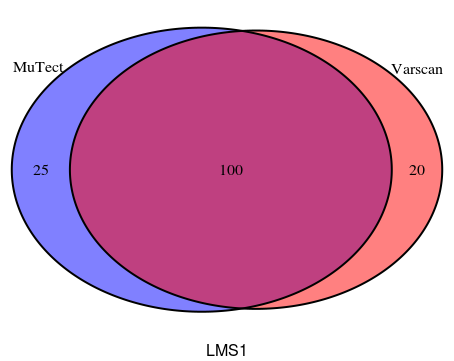
\includegraphics[scale=0.6]{Figures/LMS1.png}
\end{subfigure} 
\hspace{2.5cm}
{\vrule height 3cm width 0.1mm} 
\hspace{1cm}
\begin{subfigure}{0.4\textwidth}
\centering
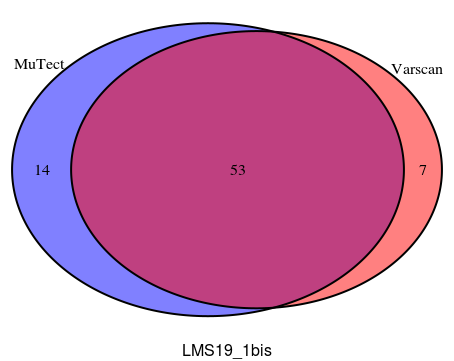
\includegraphics[scale=0.6]{Figures/LMS19_1bis.png}
\end{subfigure}
\captionsetup{justification=centering}
\caption{Nombre de mutations communes à \textbf{MuTect} et \textbf{Varscan} pour 2 échantillons de la cohorte}
\label{fig:venn}
\end{figure}

Le nombre de variants détectés par les deux logiciels varie d'un échantillon à l'autre.  Dans l'exemple de la figure \ref{fig:venn}, pour un total de 125 variations détectées dans le LMS1, 100 sont détectées à la fois par \textbf{MuTect} et par \textbf{Varscan}, soit 66\% du total. Dans le cas du LMS19T1bis, ce taux monte à 72\%.

En moyenne, 84\% des variations sont détectées par les deux logiciels. J'utilise l'intersection des deux résultats pour obtenir les mutations les plus probables.

\newpage

Je formule l'hypothèse que le nombre de mutations ne dépend pas de la localisation tissulaire des tumeurs. L'histogramme \ref{fig:mut} présente le nombre de variations qui ont été détectées et sélectionnées par les deux logiciels pour chacun des cas. 

\begin{figure}[h]
\centering
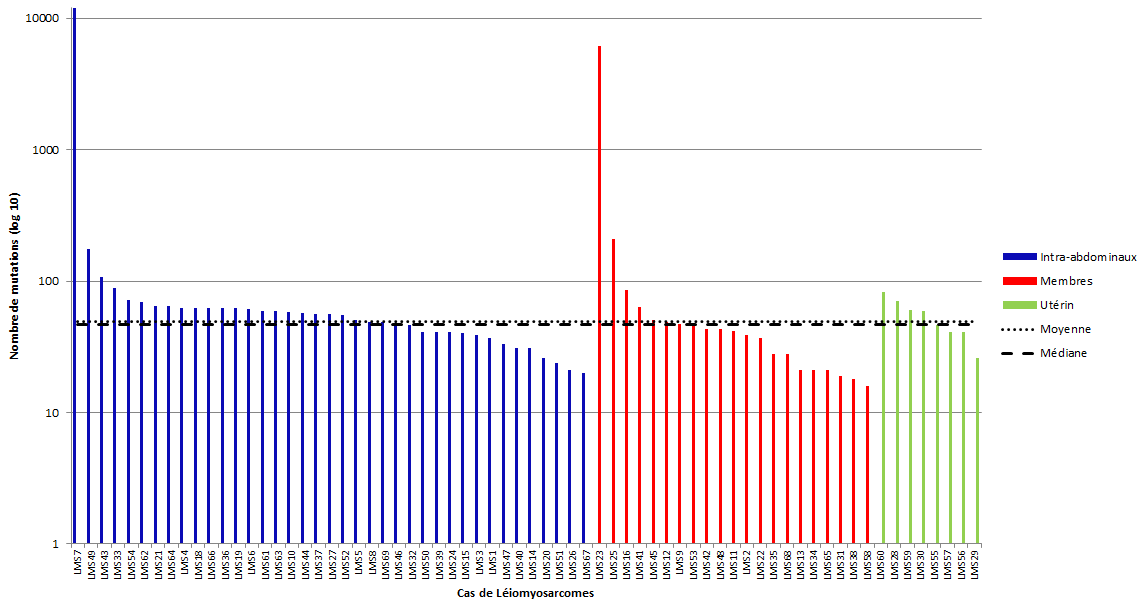
\includegraphics[width=18cm,height=12cm]{Figures/mutations.png}
\captionsetup{justification=centering}
\caption{Nombre de TFBS mutés par cas \\ 
\textit{Cas triés par type de localisation}}
\label{fig:mut}
\end{figure}

Je constate qu'il y a en moyenne 50 mutations par cas de LMS, quelle que soit la localisation. Il ne semble pas y avoir de corrélation entre le nombre de mutations des TFBS et la localisation du LMS, l'hypothèse peut être retenue.

Les cas 7, 23 et 25 se distinguent des autres par un nombre de mutations nettement supérieure à la moyenne (calculée sans ces échantillons). Pour les cas 23 et 25 la majeure partie des mutations sont du type CC$\rightarrow$TT. De telles mutations sont la signature d'une exposition aux UV \citep{signature}. Ces deux échantillons proviennent respectivement du cuir chevelu et du bras, deux zones pouvant être exposées au soleil, c'est pourquoi leurs mutations portent majoritairement la signature des UV.
Le cas 7 ne peut être expliqué par les annotations cliniques actuelles, une étude plus approfondie devra être réalisée.

Pour la suite des analyses, ces trois cas ont été mis de côté car ils représentent des cas particuliers pouvant altérer les résultats statistiques.

Les différents cas analysés ayant été prélevés à différentes localisations, il m'est possible d'étudier l'impact de cette localisation sur le nombre de TFBS mutés pour chacune des trois catégories (Intra-abdominale, Utérine, Membres).

\newpage

Le nombre de mutations des TFBS identifiées dans chaque cas en fonction de la localisation tissulaire de la tumeur est étudié. Les \og boxplots\fg ~de la figure \ref{fig:mut_n} présentent les résultats de cette étude.

\begin{figure}[h]
\centering
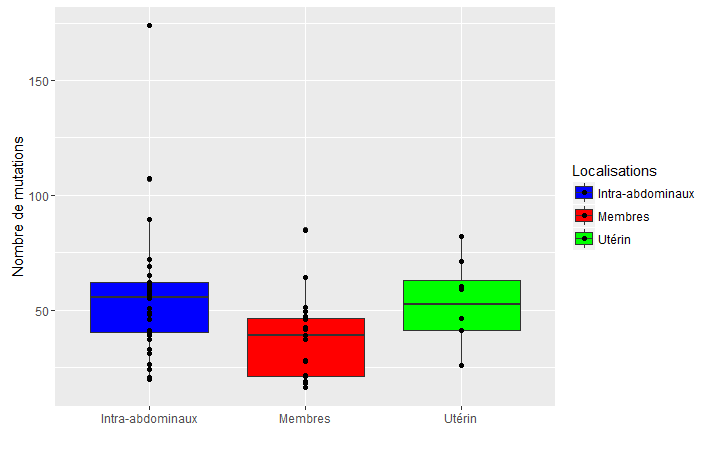
\includegraphics[scale=0.5]{Figures/number_mutations.png} 
    \caption{Variabilité du nombre de mutations en fonction de la localisation} 
    \label{fig:mut_n}
\end{figure} 

Il semble qu'il y a plus de mutations dans les échantillons intra-abdominaux et utérin que dans les membres. Cependant, le nombre de cas est très différent pour chacune des conditions (38 intra-abdominaux, 19 membres et 8 utérins), il est donc difficile de conclure précisément que la localisation de la tumeur a un impact sur le nombre de mutations.

Afin de confirmer les résultats précédents, des tests statistiques sont nécessaires. Ces tests peuvent être paramétriques (ex : t-test) ou non paramétriques (ex : Wilcoxon). Je détermine si l'échantillon suit une loi normale pour savoir quel test réaliser. Les résultats du test de normalité sont présentés sur la figure \ref{fig:shap}. 

\begin{figure}[h]
\centering
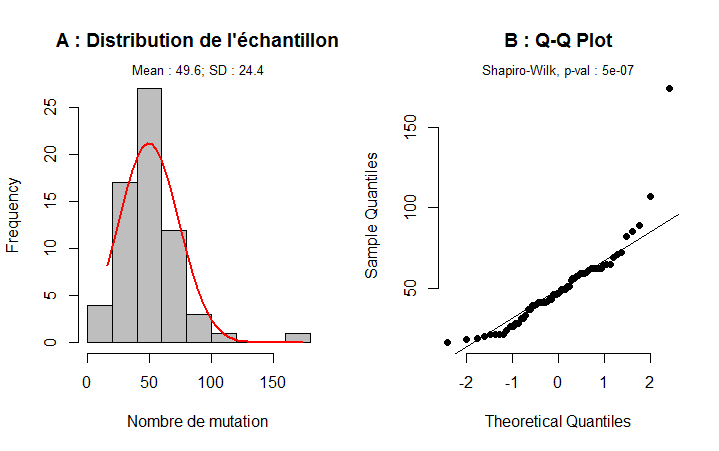
\includegraphics[width=15cm,height=8cm]{Figures/shapiro.png}
\captionsetup{justification=centering}
\caption{Test de normalité \\ 
\textit{A : Répartition du nombre de mutations dans la cohorte, B : Distribution de la cohorte par rapport à la loi normale}}
\label{fig:shap}
\end{figure}

La courbe rouge (\ref{fig:shap}.A) représente la densité de répartition des cas, elle n'est pas Gaussienne donc la population ne suit pas une loi normale. Le diagramme quantiles-quantiles (\ref{fig:shap}.B) montre que la distribution empirique des cas ne corrèle pas celle de la loi normale. De plus, la p-value est significative (p-val = $5E^{-0.7}$), l'hypothèse nulle selon laquelle la population suit une loi normale est rejetée.

Pour déterminer s'il y a une différence significative du nombre de mutations des TFBS entre les localisations, je fais un test de Wilcoxon sur échantillons appariés.

L'hypothèse nulle est qu'il n'y a pas de différence significative entre le nombre de mutations dans les échantillons et la localisation des tumeurs. Le tableau \ref{tab:wilc} contient les p-values obtenues à l'issue du test de Wilcoxon.

\begin{table}[h]
\centering
\begin{tabular}{l|c|c|}
\cline{2-3} & Intra-abdominaux & Membres\\
\hline
\multicolumn{1}{|l|}{Membres} & 0.014 & - \\
\hline
\multicolumn{1}{|l|}{Utérins}  & 0.052 & 0.185 \\
\hline
\end{tabular}
\caption{p-value du test de Wilcoxon}
\label{tab:wilc}
\end{table}

Lorsque je compare l'ensemble des échantillons intra-abdominaux et des membres, la p-value est significative (p-val = 0.014), l'hypothèse nulle est donc rejetée. La localisation des tumeurs a une influence sur le nombre de variations.

Les p-values observées lors de la comparaison des échantillons intra-abdominaux ou membres ou utérins montre  qu'il n'y a pas d'influence de la localisations des tumeurs sur le nombre de variations.

Les analyses statistiques montrent que la localisation peut être corrélée au nombre de mutations des TFBS dans chaque échantillon. La suite de mes analyses portent donc sur le nombre de cas présentant des mutations pour les TFBS de chaque facteur de transcription et ce indépendamment de leur localisation.

\section{Caractérisation des mutations}

Je me suis intéressée aux pourcentages d'échantillons portant des mutations des TFBS pour chacun des facteurs de transcription. La figure \ref{fig:pourcent} présente ces pourcentages. 

\begin{figure}[h]
\centering
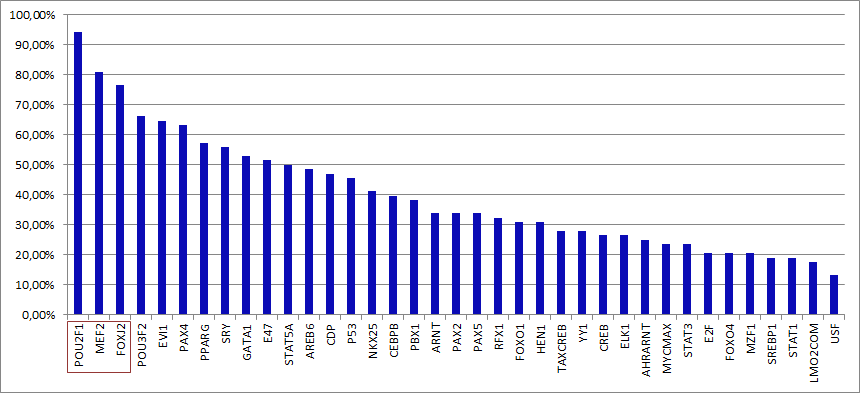
\includegraphics[scale=0.7]{Figures/pourcentage.png}
\captionsetup{justification=centering}
\caption{Pourcentage de cas mutés pour chaque facteur de transcription présentant des TFBS mutés}
\label{fig:pourcent}
\end{figure}

Je constate que les TFBS du facteur de transcription POU2F1 sont mutés dans plus de 90\% des cas, et ceux de MEF2 et de FOXJ2 sont mutés dans plus de 70\% des cas.  Ces trois facteurs de transcription ont respectivement des rôles dans  l'expression du  gène récepteur de la gonadotropine, l'activation de la myogénèse et la migration cellulaire. Des altérations de ces trois facteurs ont été observées dans d'autres cancers. La sur-expression de FOXJ2 diminue la migration cellulaire dans le cancer du sein \citep{foxj2_cancer},la sur ou sous expression de POU2F1 dérégule les fonctions souches des cellules normales et cancéreuses de tous les tissus \citep{oct1_cancer}, la sous-expression de MEF2 entraîne l'augmentation de la prolifération cellulaire \citep{mef2_cancer}. J'ai donc focalisé la suite de mes analyses sur ceux-ci.

Le tableau \ref{fig:tf}, regroupe le nombre de mutations des TFBS pour chacun des trois facteurs de transcription précédemment cités. J'ai sélectionné un échantillon de 6 cas différents de LMS (2 intra-abdominaux, 2 membres et 2 utérins) au hasard parmi les 68. 

\begin{figure}[h]
\renewcommand{\figurename}{Tableau}
\centering
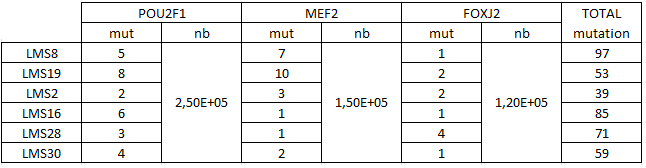
\includegraphics[scale=1]{Figures/table.png}
\captionsetup{justification=centering}
\caption{Nombre de TFBS mutés pour POU2F1, MEF2 et FOXJ2\\
\textit{mut : nombre de mutations, nb : nombre total de TFBS existant pour ce facteur, TOTAL : nombre de TFBS mutés dans l'échantillon}}
\label{fig:tf}
\end{figure}

Je constate que pour chaque cas, il y a en moyenne 4.5 TFBS de POU2F1 mutés dans le même échantillon (4 pour MEF2 et 1.8 pour FOXJ2). 

Ces résultats sont purement prédictifs, des analyses biologiques doivent être réalisées pour les vérifier. J'ai sélectionné trois mutations situées, chacune provenant d'un LMS différent (LMS5,LMS9 et LMS29) et étant placée au milieu du TFBS car lorsque la mutation est située en périphérie elle risque de toucher une autre portion du génome. Ces trois mutations ont été transmises aux biologistes de l'équipe pour une vérification expérimentale.

Cette vérification se déroule en deux étapes. La première est une analyse \og Polymerase Chain Reaction\fg durant laquelle la séquence d'intérêt est amplifiée. La seconde est un séquençage de l'ADN par la méthode Sanger. 

Le résultat de cette analyse pour le LMS5 est présenté sur la figure \ref{fig:oct}.

\begin{figure}[h]
\centering
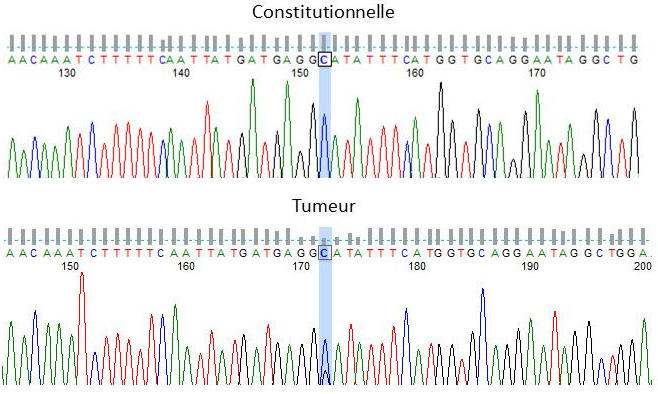
\includegraphics[width=15cm,height=6.5cm]{Figures/OCT1.jpg}
\captionsetup{justification=centering}
\caption{Chromatogramme des séquences d'ADN constitutionnel et tumoral du LMS5
\\ \textit{haut : séquence constitutionnelle, bas : séquence tumorale \\ Bleu : position de la mutation étudiée}}
\label{fig:oct}
\end{figure}

Je constate que sur le \gls{chromatogramme} de la figure \ref{fig:oct} de la séquence tumorale une mutation C $\rightarrow$ G à la position indiquée par les analyses bioinformatiques est présente. Cette mutation est absente de la séquence constitutionnelle, elle peut être caractérisée de somatique.

Sur les trois mutations testées, les analyses biologiques sont revenues positives pour deux échantillons (le LMS5 et le LMS9). Le troisième échantillon (LMS29) présente trop de bruit de fond pour confirmer la présence de la mutation. 

J'ai constaté qu'en moyenne 3 TFBS du même facteur de transcription sont mutés dans le même échantillon (voir tableau \ref{fig:tf}). Il apparaît intéressant d'étudier l'impact de ces mutations sur les gènes cibles des facteurs de transcriptions et plus précisément sur leur expression.

Pour étudier l'expression des gènes cibles des trois facteurs de transcription sélectionnés (POU2F1, MEF2, FOXJ2), j'analyse les valeurs de FPKM pour chacun des gènes situés à proximité de chacun des TFBS mutés.

\begin{figure}[h]
\centering
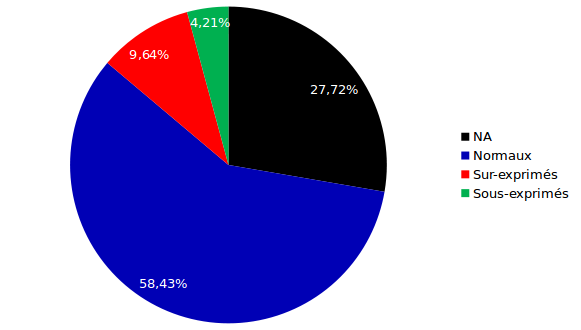
\includegraphics[scale=0.9]{Figures/Camembert.png}
\captionsetup{justification=centering}
\caption{Proportion de gènes sur ou sous exprimés \\ NA : Sans valeur de FPKM}
\label{fig:cam}
\end{figure}

Parmi tous les gènes, j'observe sur le graphique en secteurs (figure \ref{fig:cam}) que 31\% n'ont pas de valeur de FPKM. Ils correspondent à des pseudogènes ou des gènes non-codant, ils ne sont pas présents dans les données de transcriptome qui servent au calcul du FPKM et n'ont donc aucune valeur.

Dans 56\% des cas, les gènes n'ont pas de changement d'expression. Il est possible que ces gènes ne soient pas des cibles du facteur de transcription pour lequel le TFBS est muté ou qu'un autre facteur de transcription compense. Une troisième hypothèse serait qu'un autre facteur de transcription se soit fixé sur le site muté et qu'il joue un rôle similaire sur le même gène.

Parmi les gènes récupérés à proximité des TFBS mutés, seulement 13\% sont sur-exprimés ou sous-exprimés. Parmi ces gènes se trouvent des gènes cibles, il est possible que la différence d'expression de ceux ci soit liée à la mutation du TFBS.

\newpage
Les gènes cibles des facteurs de transcription sont contenus dans deux bases de données (partie \ref{subsec:identification}). L'intersection de cette base avec le fichier des 10 gènes voisins des TFBS me permet de savoir combien de gènes cibles sont présents.

\begin{figure}[h]
\centering
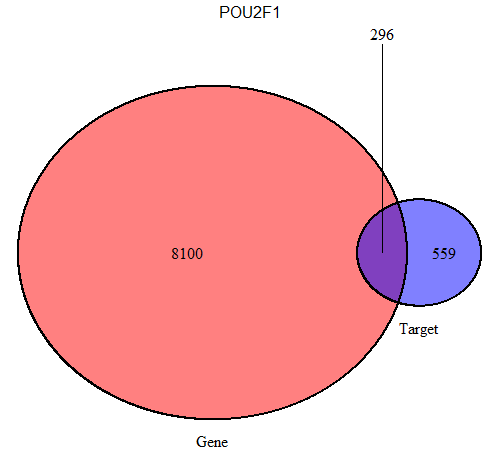
\includegraphics[scale=0.6]{Figures/POU2F1.png}
\captionsetup{justification=centering}
\caption{Nombre de gènes associés aux TFBS mutés de POU2F1 \\ Bleu : gènes cibles identifiés dans \textbf{TRANSFAC}, Rouge : 10 gènes autour de chaque TFBS}
\label{fig:pou}
\end{figure}


Dans le cas du facteur de transcription POU2F1 présenté sur la figure \ref{fig:pou}, je constate que la proportion de gènes cibles présents parmi les gènes voisins des TFBS est de 2\%. J'observe des résultats similaires pour les deux autres facteurs étudiés : MEF2 et FOXJ2.

L'analyse de la figure \ref{fig:cam} m'a permis d'identifier des gènes sur ou sous exprimés autour des TFBS. Sur l'ensemble de ces gènes, certains sont des gènes cibles du facteur de transcription étudié (figure \ref{fig:pou}). Je m'intéresse alors à la proportion de gènes sur ou sous exprimés étant également des gènes cibles.

\begin{figure}[h]
\centering
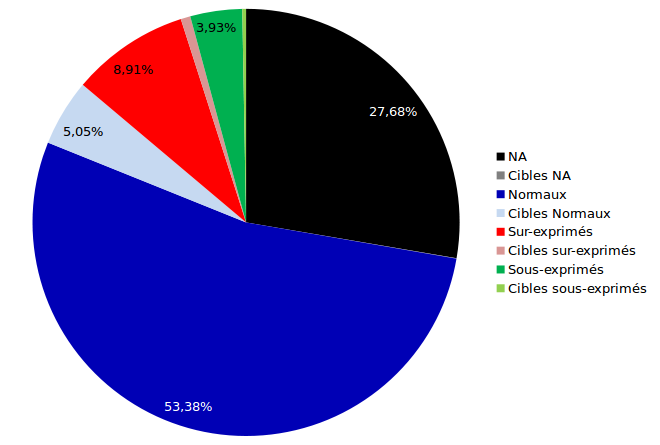
\includegraphics[scale=0.7]{Figures/Cible_expression.png}
\captionsetup{justification=centering}
\caption{Proportion de gènes cibles en fonction de l'expression\\
\textit{Sur tous les TFBS et tous les échantillons}}
\label{fig:pou}
\end{figure}

Parmi tous les gènes proches des TFBS, j'observe que 5.05\% des gènes n'ayant pas de changement d'expression sont des gènes cibles. L'expression des gènes étant régulés par plusieurs facteurs de transcription, il est possible qu'il y ait eu un phénomène de compensation via un autre facteur.

Une faible proportion des gènes sur-exprimés (0.73\%) et des gènes sous-exprimés (0.28\%) sont également des gènes cibles, soit 92 gènes sur les 9169 récupérés autour des TFBS. Dans ces deux cas, il est possible que la mutation du TFBS ait empêcher le bon fonctionnement du facteur de transcription associé.

Les rôles de ces 92 gènes dans le programme transcriptionnel sont variés. Une analyse de l'ontologie de ces gènes (GO) permet de connaître les différents rôles. La figure \ref{fig:go} présente le résultat de cette analyse pour les 20 éléments les plus représentatifs (p-value ajustée Benjamini-Hochberg).

\begin{figure}[h]
\centering
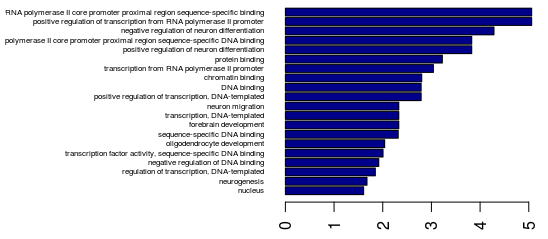
\includegraphics[scale=1]{Figures/GO.png}
\captionsetup{justification=centering}
\caption{Analyse d'enrichissement des gènes cibles de POU2F1, MEF2 et FOXJ2}
\label{fig:go}
\end{figure}

La majeure partie de ces gènes sont impliqués dans les régulations de la transcription au niveau du promoteur de l'ARN polymérase II lequel permet la formation du complexe d'initialisation. D'autres sont impliqués dans la différenciation cellulaire ou la fixation des différents éléments du génome (chromatine, protéine, ADN) ou encore dans la régulation de la différenciation neuronale.

L'hypothèse de départ est que les mutations des TFBS peuvent avoir un impact sur l'expression des gènes cibles des facteurs de transcription qui leurs sont associés. 

L'analyse des TFBS démontre que, quelle que soit la localisation des tumeurs, le nombre de mutations reste le même (en moyenne 50). J'ai également observé que plusieurs TFBS d'un seul facteur de transcription peuvent être mutés dans le même échantillon, ces mutations étant toutes uniques.

L'analyse des gènes proches des TFBS mutés démontre que très peu de ces gènes présentent un changement d'expression. Cependant, parmi tous les gènes récupérés, une partie importante concerne des gènes non codant ou des pseudogènes, il faudra donc refaire les analyses en les intégrant dans l'analyse RNASeq initiale. 

Dans les gènes présentant un changement d'expression se trouve des gènes cibles, il semble donc que l'hypothèse de départ soit validée. Des mutations somatiques dans les TFBS pourraient avoir un impact sur l'expression des gènes cibles des facteurs de transcription qui leurs sont associés. Pour vérifier cette hypothèse, il faudra récupérer l'expression basale des gènes, via des projet comme \textbf{ENCODE}. Cette expression sera comparée à l'expression retrouvée dans les échantillons mutés.

Des analyses \og Chip Seq\fg ~pourront être réalisées afin de déterminer si le facteur de transcription se fixe à son TFBS dans l'échantillon constitutionnel et ne se fixe plus dans la tumeur. En effet, si le facteur ne se fixe pas dans l'échantillon constitutionnel, le changement d'expression du gène cible ne résulte pas de la mutation du TFBS.

\addcontentsline{toc}{chapter}{Conclusion}
\chapter*{Conclusion}

L'objectif principal de mon travail était d'identifier et de caractériser les modifications du programme transcriptionnel associées à des mutations somatique des TFBS dans les léiomyosarcomes. Un pipeline d'analyses de données a été réalisé afin d'extraire les mutations somatiques des TFBS, il a pu être lancé sur les 80 échantillons des 68 cas actuellement disponibles. 

Il ressort qu'en moyenne, chaque échantillon possède 50 mutations différentes des TFBS et ce quelle que soit la localisation de la tumeur. Pour des raisons techniques et logistiques, seulement trois de ces mutations, chacune appartenant à un léiomyosarcome différent, ont pu être testées. Il faudra donc étendre les vérifications à un plus grand nombre de mutations et si possible à tous les échantillons pour juger de la viabilité des résultats. 

Dans les échantillons, j'ai pu observer que les mutations des TFBS sont très peu nombreuses (0.05\%) ce qui correspond aux observations de \citeauthor{Melton}. 92 gènes cibles des facteurs de transcription POU2F1,MEF2 et FOXJ2 associés à des mutations des TFBS présentent des changements d'expression. Ces différents gènes modifie le programme transcriptionnel en jouant sur la fixation de l'ADN, des protéines, de l'ARN polymérase II ou encore dans la différenciation neuronale. 

De telles modifications pourraient être à l'origine du développement de tumeurs. Les gènes n'étant pas mutés, il faudra réaliser des analyses \og Chip Seq\fg afin de savoir si le facteur de transcription associé au site muté s'y fixe. Dans le cas d'une non fixation au niveau de la tumeur, l'hypothèse sera que la modification d'expression du gène est lié à la mutation du TFBS. 

L'équipe \textit{Génétique et biologie des sarcomes} dirigée par Frédéric Chibon devrait débuter la seconde phase du projet \og Soft tissue cancer\fg ~cette année, en complétant le jeu de données afin d'obtenir une cohorte d'au moins 200 cas. Le pipeline d'analyse pourra être exécuté sur ces nouveaux cas afin de confirmer ou d'infirmer les observations précédentes. De même, les mutations détectées pourront par la suite être validées ou invalidées par des analyses biologiques.

Les test statistiques réalisés lors de mon projet ont été réalisés sur un faible nombre d'échantillons. Il faudra donc les confirmer ou les infirmer en utilisant les nouveaux cas issus de la seconde phase du projet. Pour obtenir des résultats optimaux, il faudra avoir une répartition équitable des échantillons pour chaque localisation.

Les bases de données des gènes cibles utilisées ne contiennent que des données vérifiées biologiquement. Pour compléter le nombre de gènes cibles, il faudra utiliser des bases de données prédictives.

Les gènes récupérés autour des TFBS mutés peuvent être des oncogènes ou des suppresseurs de tumeurs déjà connus. Une analyse de ces gènes pourra donc permettre de ressortir des éléments déjà observés dans la littérature et ainsi orienter les futures analyses sur les éléments jusqu'alors inconnus.






\appendix
\titleformat{\chapter}[frame]
  {\huge\normalfont\sc} 
  {\filright\footnotesize\enspace ANNEXE \thechapter\enspace}  {8pt}
  {\filcenter} 
\addcontentsline{toc}{chapter}{Annexes}
\renewcommand{\thefigure}{A\arabic{figure}}
\setcounter{figure}{0}

\chapter*{Annexes}

\renewcommand{\figurename}{Annexe}
\begin{figure}[h]
  \begin{adjustbox}
  {
  addcode=
  	{\begin{minipage}{\width}}
  		{\caption{Illustration des types de mutations}
         \label{fig:somatique}
    \end{minipage}},
  rotate=90,
  center
  }
    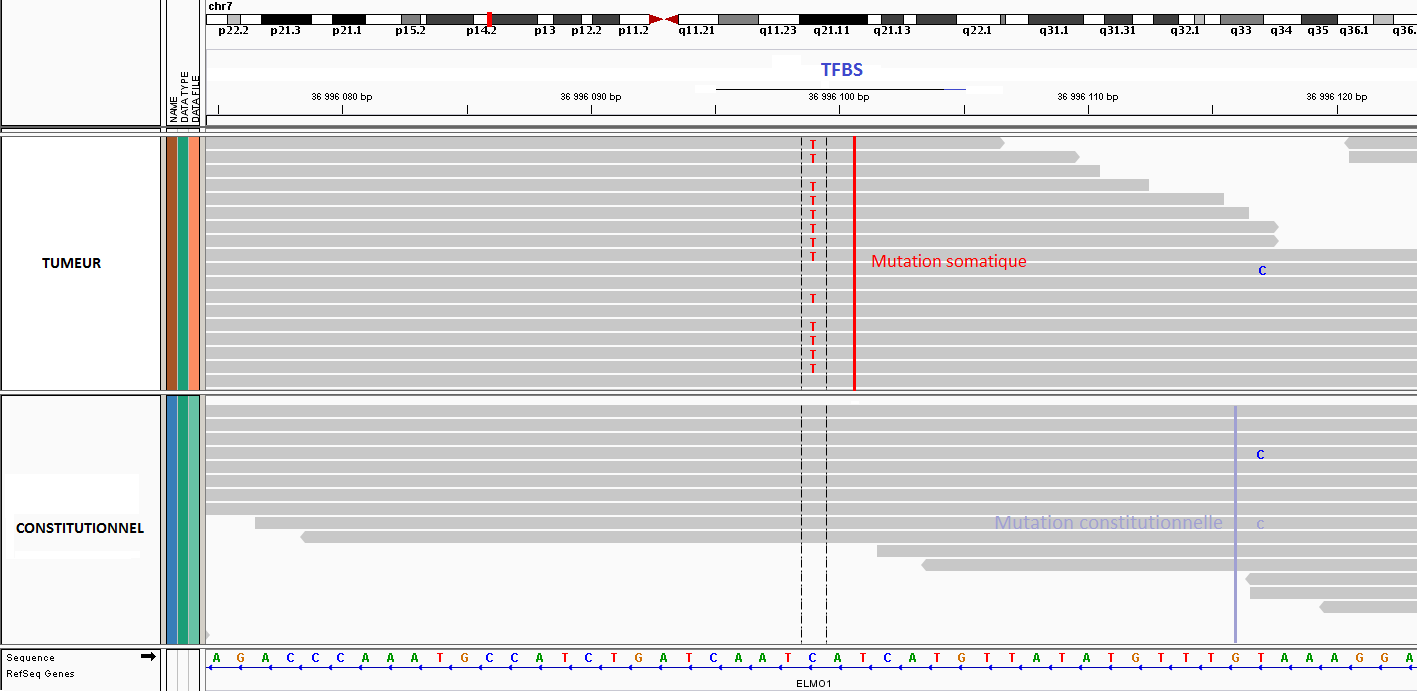
\includegraphics[height=15cm,width=21cm]{Figures/mutation.png}
  \end{adjustbox}
\end{figure}



\printglossary[title={Glossaire}, toctitle={Glossaire}]

\bibliographystyle{plainnat} % or try abbrvnat or unsrtnat
\bibliography{Bibliographie/biblio} % refers to example.bib
\addcontentsline{toc}{chapter}{Bibliographie}

\end{document}